% !TEX root = thesis.tex

%%
%%
%% Results chapter
%%
%%

This chapter describes the results of several experiments, each run with a variation of the setup.
In each case, we compare the results of 1,000 simulations using several error functions.
The results of the first experiment, uniform population and a uniform intensity,
are described in \autoref{sec:results:unif_100_unif}.
We then made ran several sets of experiments while changing one parameter at a time.
\autoref{sec:results:unif_NCases_1h} compares the results obtained by varying the number of cases.
\autoref{sec:results:unifNpop_1h} compares the results obtained by varying the size of the population.

\textbf{
\color{red}
This table shows that the method is not consistent.
There is an issue with the CV using gradient descent.
However, even the Oracle and Silverman bandwidths have INCREASING normalized error.
Also note the bandwidths are getting smaller.
}

$$
\lambda(\vec{x}) = \mu f\!(\vec{x})
$$

where $\mu$ is a constant multiplier.
Normalized MISE is MISE divided by $\mu$.

\textbf{
    \color{red}
    Also note that taking the average of the 2 Oracle bandwidths for $\mu=1$ is 1.35,
    and $1.35 \mu^{-1/6}$ gives:
    \\
    1.5153238 \\
    1.3500000 \\
    1.2027133 \\
    1.0323781 \\
    0.9197443
}

% latex table generated in R 3.3.3 by xtable 1.8-2 package
% Tue Jan 16 19:25:44 2018
\begin{table}[ht]
\centering
\small
\color{red}
\begin{tabular}{rrrrrrr}
  \hline
mu & oracle.nmise & silverman.nmise & cv.nmise & oracle.best\_h1 & oracle.best\_h2 & silverman.mean\_h \\ 
  \hline
0.500000 & 0.000018 & 0.000029 & 0.000028 & 1.500000 & 1.500000 & 1.033278 \\ 
  1.000000 & 0.000022 & 0.000035 & 0.000033 & 1.300000 & 1.400000 & 0.918091 \\ 
  2.000000 & 0.000026 & 0.000042 & 0.000036 & 1.200000 & 1.200000 & 0.817562 \\ 
  5.000000 & 0.000034 & 0.000053 & 0.000058 & 1.100000 & 1.000000 & 0.703114 \\ 
  10.000000 & 0.000038 & 0.000062 & 0.000114 & 0.900000 & 0.900000 & 0.626736 \\ 
   \hline
\end{tabular}
\end{table}

%%%%%%%%%%%%%%%%%%%%%%%%%%%%%%%%%%%%%%%%%%%%%%%%%
% Results template
%%%%%%%%%%%%%%%%%%%%%%%%%%%%%%%%%%%%%%%%%%%%%%%%%
\section*{Results template}
\label{sec:results:template}
\graphicspath{{./results/unif_100_1.0_1h/}}
\makeatletter
\def\input@path{{./results/unif_100_1.0_1h/}}
\makeatother

%%%%%%%%%%%%%%%%%%%%%%%%%%%%%%%%%%%%%%%%%%%%%%%%%
% Parameter table - template
%%%%%%%%%%%%%%%%%%%%%%%%%%%%%%%%%%%%%%%%%%%%%%%%%
\begin{table}[htbp]
\centering
\begin{tabular}{ll}
\hline
Parameter & Value \\
\hline
Population size & 10,000 \\
Population decay rate & uniform \\
Incident risk factor & 100 \\
Incident decay rate & uniform \\
Incident center & -- \\
\hline
\end{tabular}
\caption{Parameters used in TEMPLATE}
\label{tab:params:template}
\end{table}

%%%%%%%%%%%%%%%%%%%%%%%%%%%%%%%%%%%%%%%%%%%%%%%%%
% Example cases scatter - template
%%%%%%%%%%%%%%%%%%%%%%%%%%%%%%%%%%%%%%%%%%%%%%%%%
\begin{figure}[htbp]
    \centering
    \begin{subfigure}[t]{0.32\textwidth}
    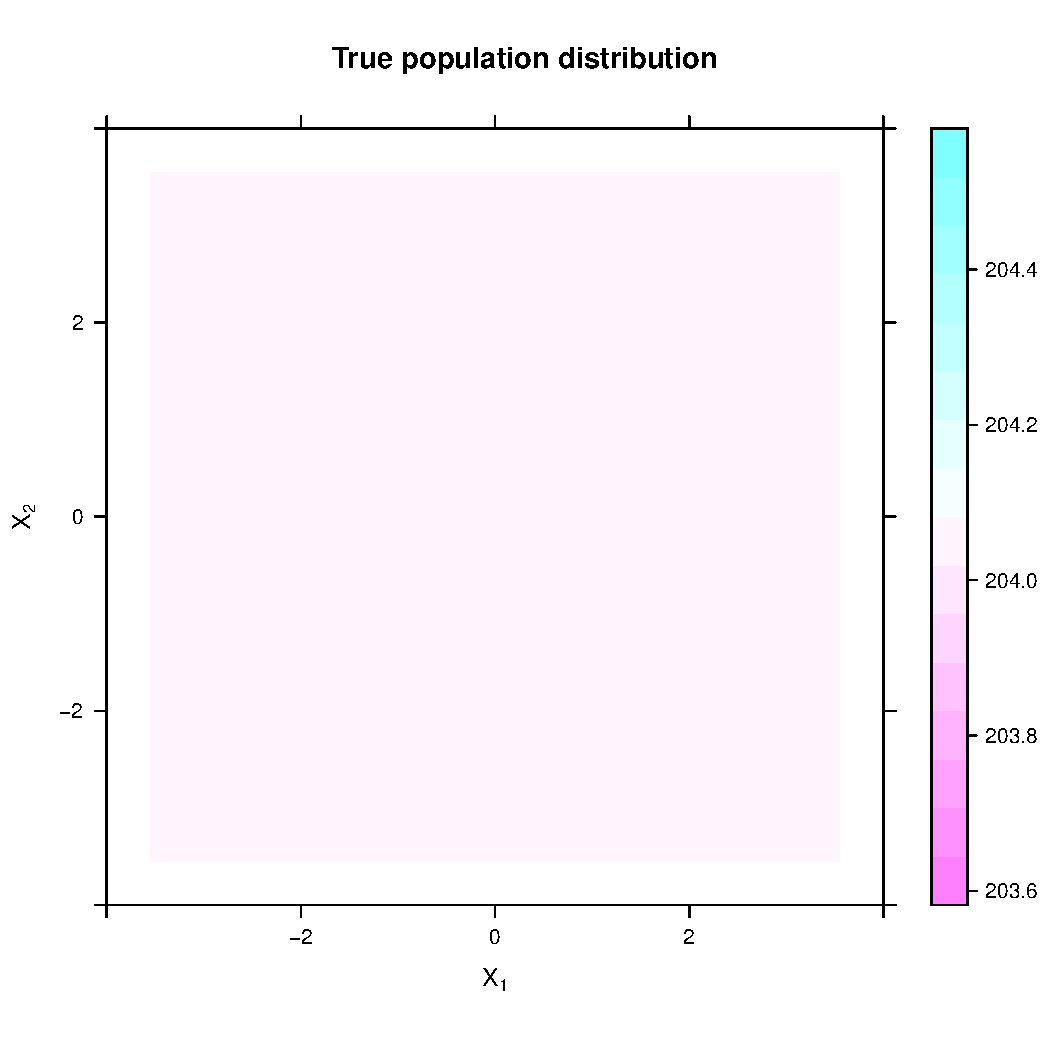
\includegraphics[width=\textwidth]{output/population-heatmap}
    \caption{Population distribution}
    \end{subfigure}
    \begin{subfigure}[t]{0.32\textwidth}
    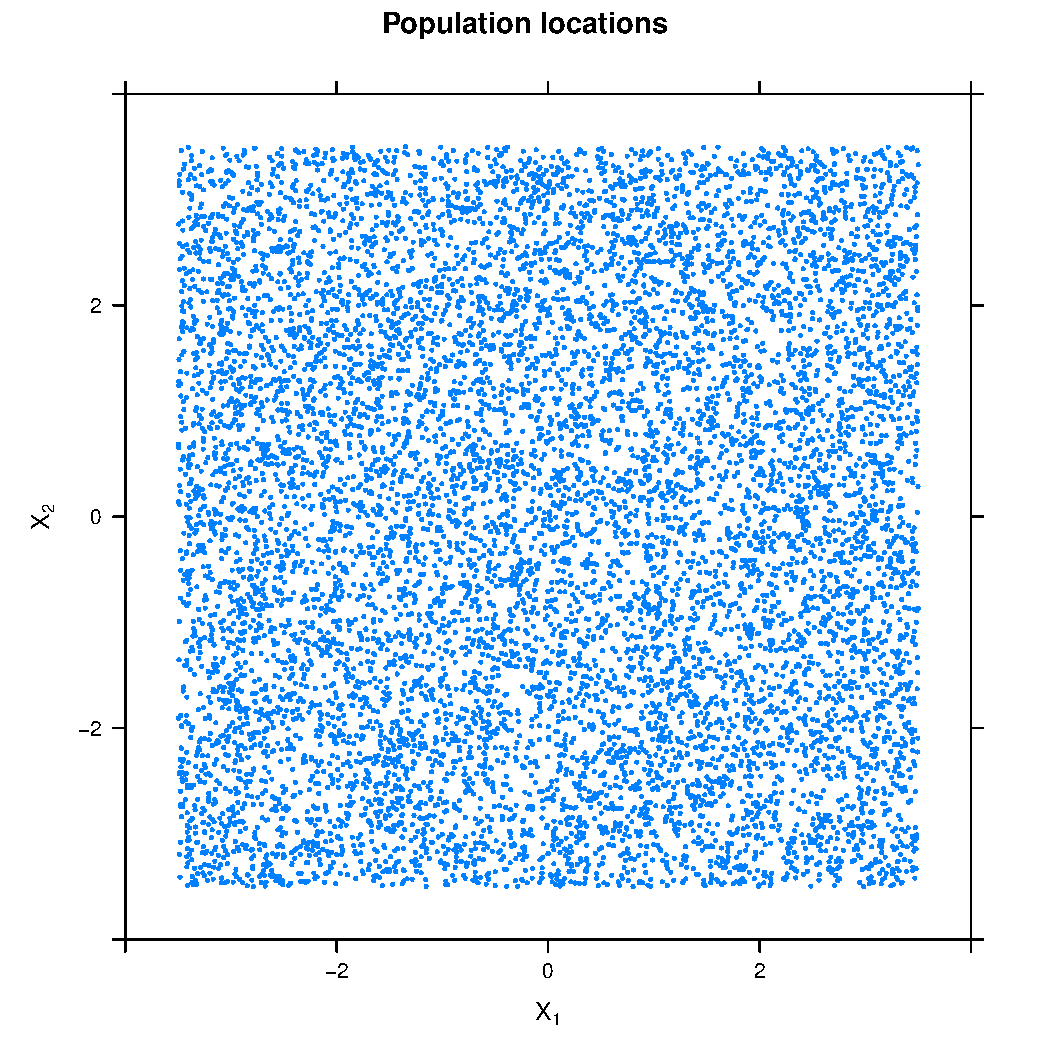
\includegraphics[width=\textwidth]{output/population-points}
    \caption{Population realization}
    \end{subfigure}%
    \begin{subfigure}[t]{0.32\textwidth}
    \includegraphics[width=\textwidth]{output/population_and_incidents_scatter}
    \caption{With incidents}
    \end{subfigure}%
    \caption[Uniform population distribution]
        {Population distribution (a), realization (b), and sample incidents (c)}
    \label{fig:cases:template}    
\end{figure}

%%%%%%%%%%%%%%%%%%%%%%%%%%%%%%%%%%%%%%%%%%%%%%%%%
% Example cases heat map - template
%%%%%%%%%%%%%%%%%%%%%%%%%%%%%%%%%%%%%%%%%%%%%%%%%
\begin{figure}[htbp]
    \centering
    \begin{subfigure}[t]{0.45\textwidth}
    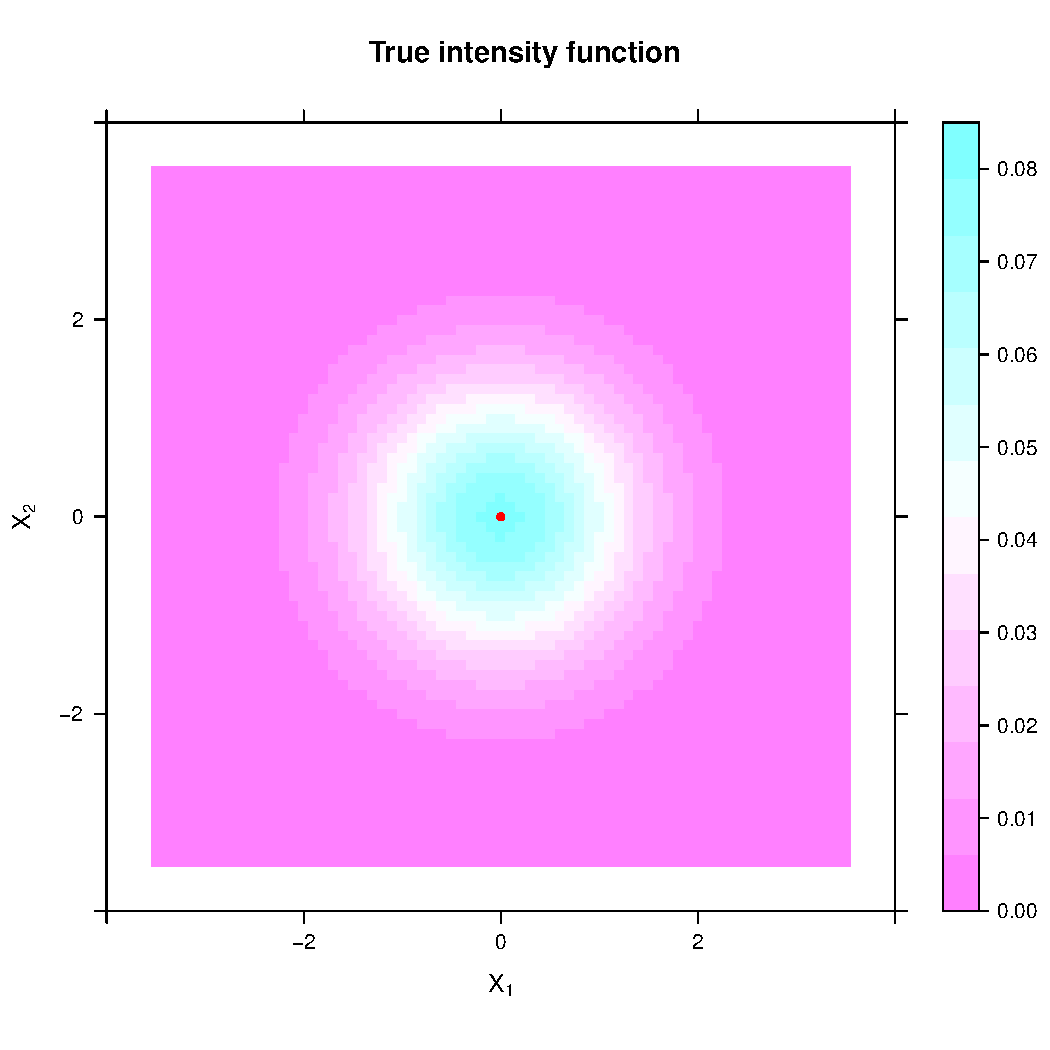
\includegraphics[width=\textwidth]{output/true_intensity_heatmap}
    \caption{True intensity}
    \end{subfigure}%
    \begin{subfigure}[t]{0.45\textwidth}
    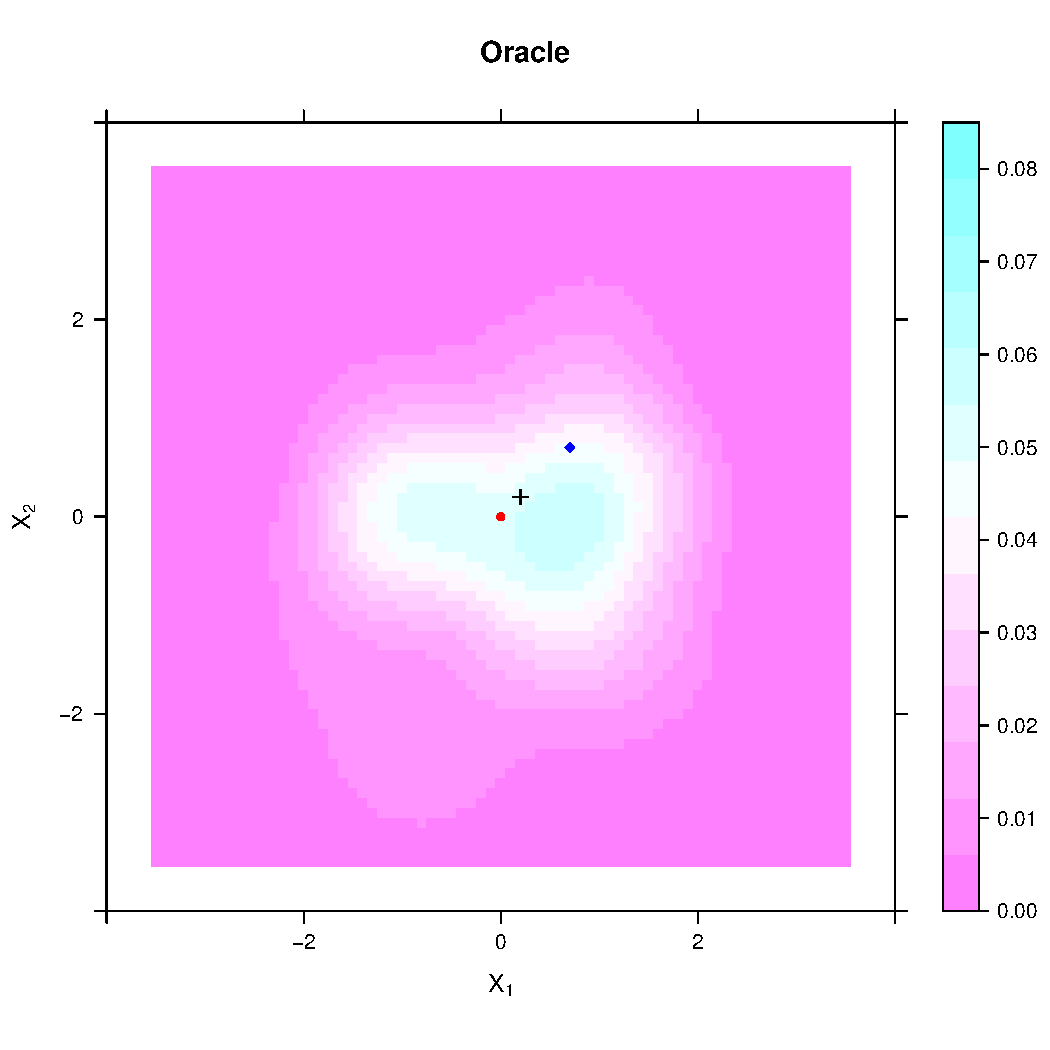
\includegraphics[width=\textwidth]{output/oracle_intensity_heatmap}
    \caption{Oracle bandwidth estimate}
    \end{subfigure}


    \begin{subfigure}[b]{0.45\textwidth}
    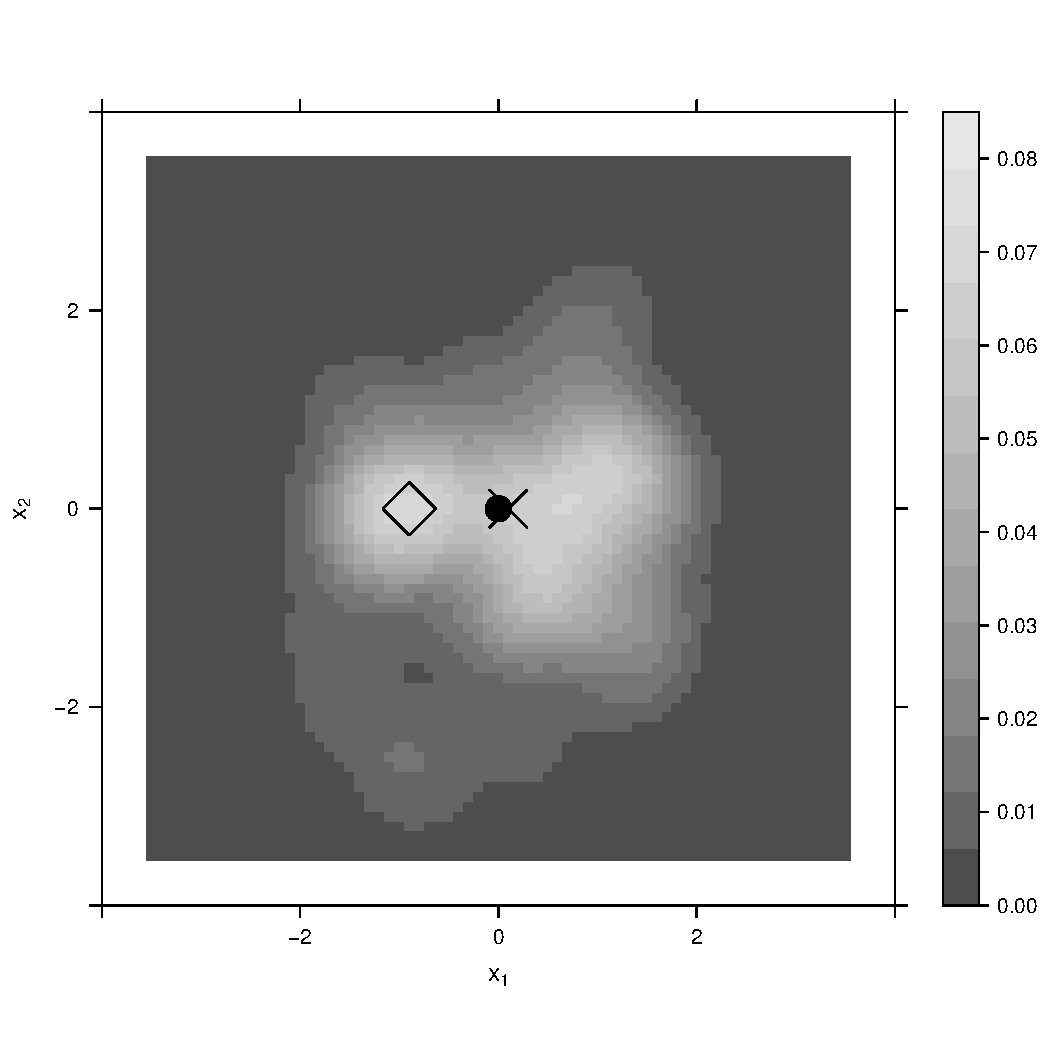
\includegraphics[width=\textwidth]{output/silverman_intensity_heatmap}
    \caption{Silverman bandwidth estimate}
    \end{subfigure}%
    \begin{subfigure}[b]{0.45\textwidth}
    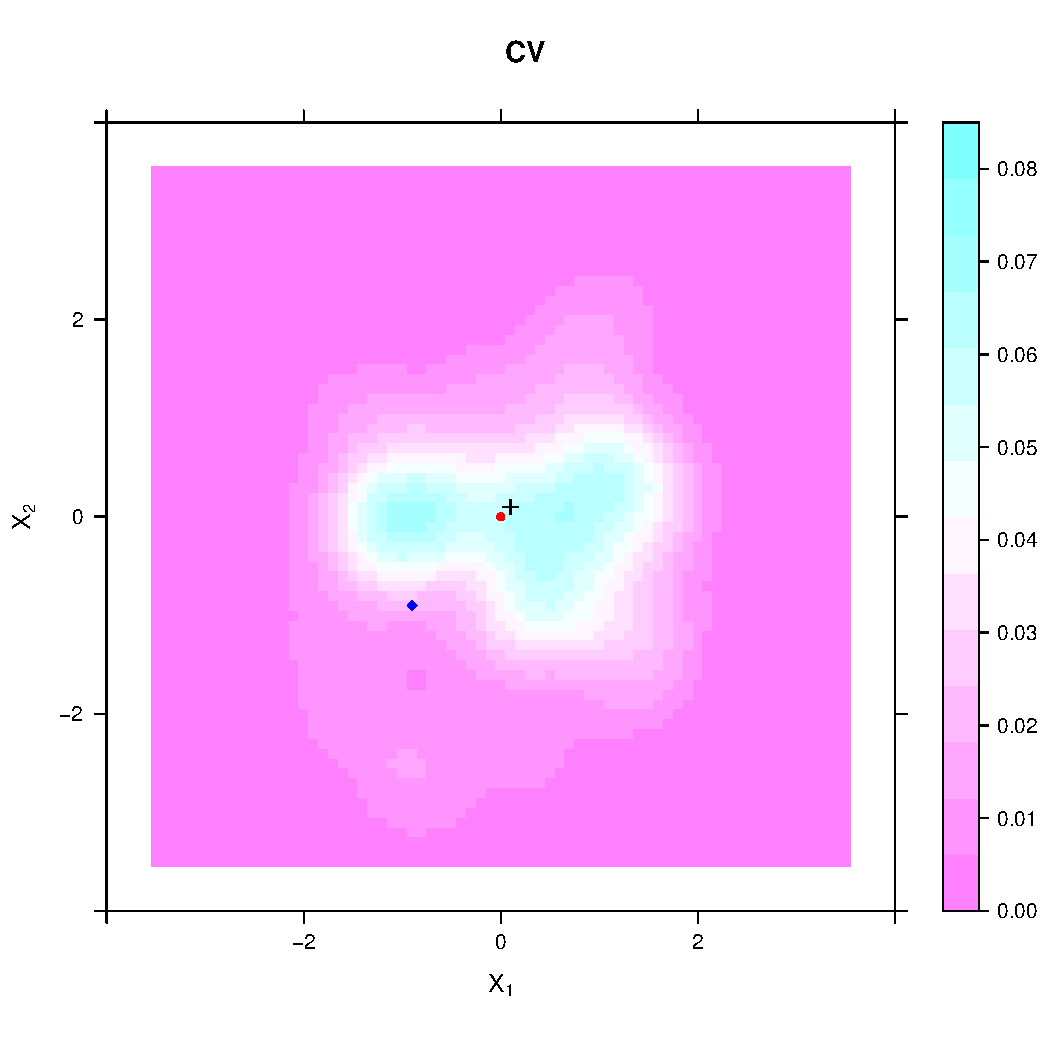
\includegraphics[width=\textwidth]{output/CV_intensity_heatmap}
    \caption{Cross-validation bandwidth estimate}
    \end{subfigure}
    \caption[Example incidents: uniform intensity on uniform population, 100 cases]
        {Example incidents: uniform intensity on uniform population, 100 cases}
    \label{fig:cases:template}
\end{figure}

%%%%%%%%%%%%%%%%%%%%%%%%%%%%%%%%%%%%%%%%%%%%%%%%%
% ISE distribution - template
%%%%%%%%%%%%%%%%%%%%%%%%%%%%%%%%%%%%%%%%%%%%%%%%%
\begin{figure}[htbp]
    \centering
    \begin{subfigure}[b]{0.45\textwidth}
    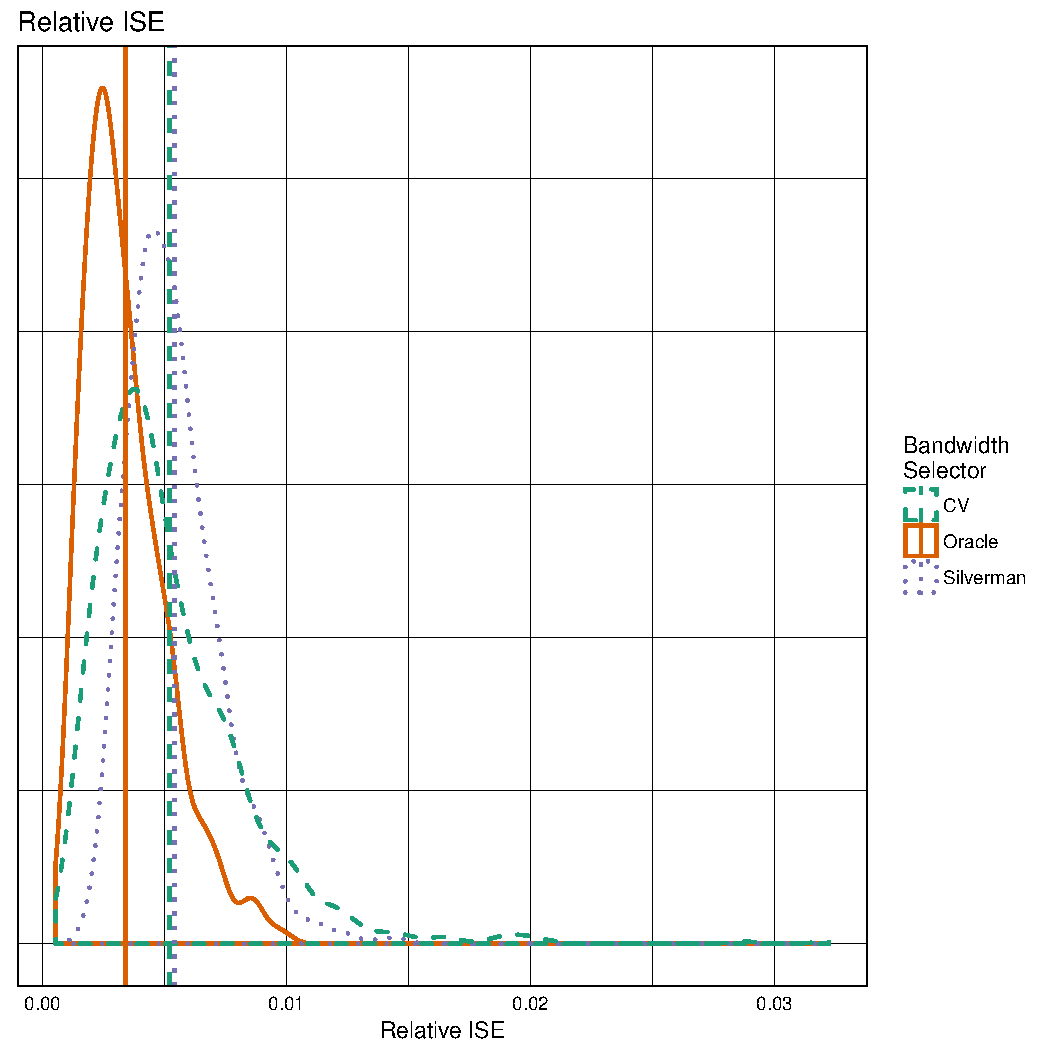
\includegraphics[width=\textwidth]{output/ise-relative-histogram}
    \caption{Relative ISE}
    \end{subfigure}
    \begin{subfigure}[b]{0.45\textwidth}
    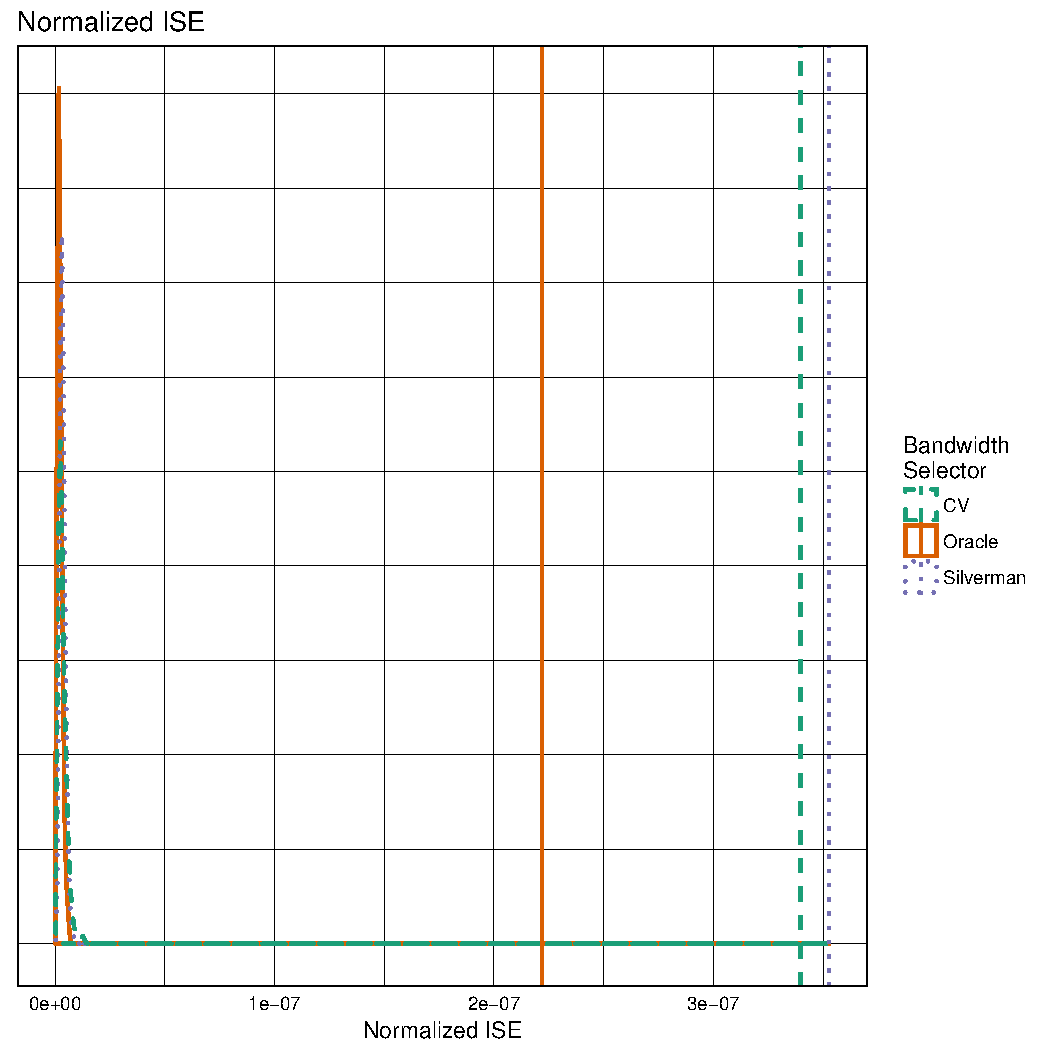
\includegraphics[width=\textwidth]{output/ise-normalized-histogram}
    \caption{Normalized absolute ISE}
    \end{subfigure}
    \caption[ISE: uniform on uniform]{Integrated squared error histogram for uniform intensity on a uniform population, 100 cases}
    \label{fig:ise:template}
\end{figure}

%%%%%%%%%%%%%%%%%%%%%%%%%%%%%%%%%%%%%%%%%%%%%%%%%
% IAE distribution - template
%%%%%%%%%%%%%%%%%%%%%%%%%%%%%%%%%%%%%%%%%%%%%%%%%
\begin{figure}[htbp]
    \centering
    \begin{subfigure}[b]{0.45\textwidth}
    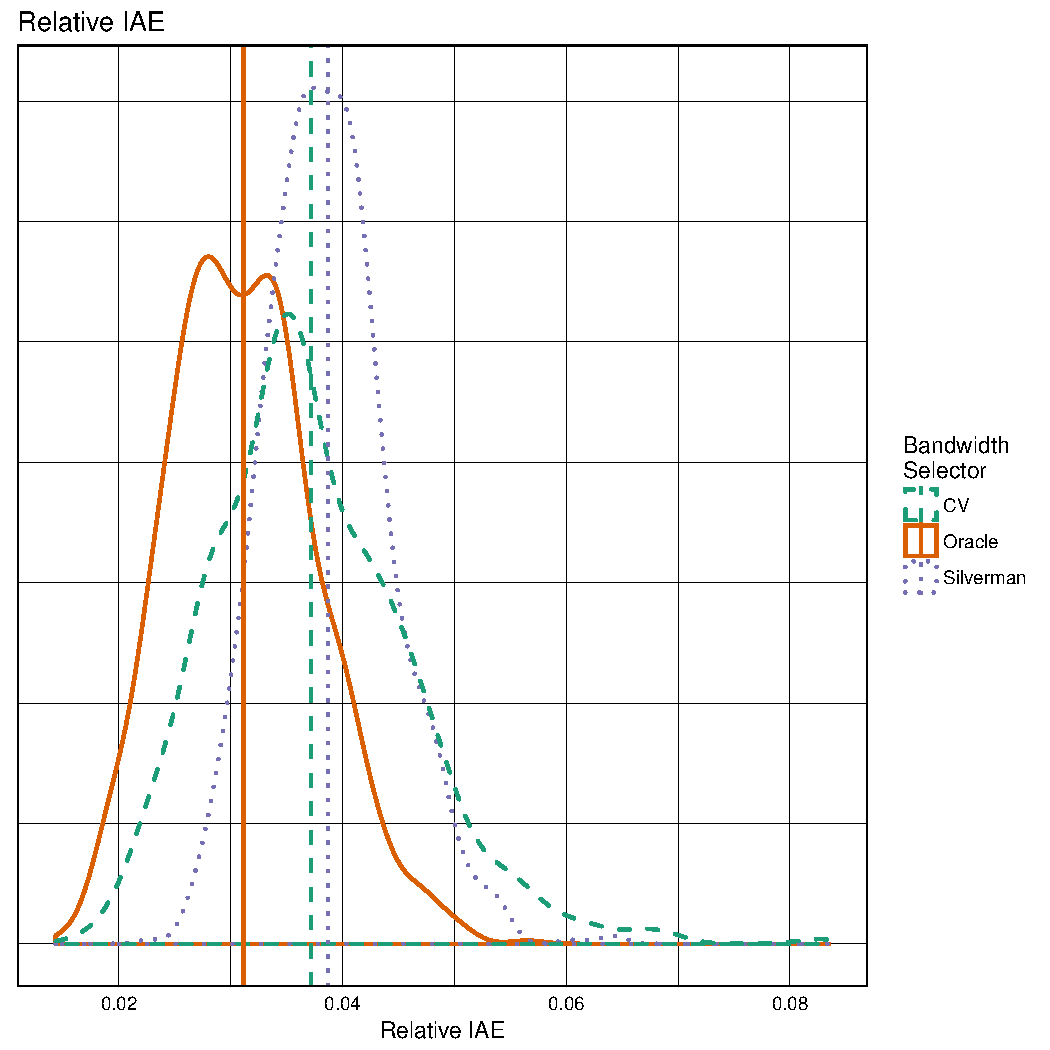
\includegraphics[width=\textwidth]{output/iae-relative-histogram}
    \caption{Relative IAE}
    \end{subfigure}
    \begin{subfigure}[b]{0.45\textwidth}
    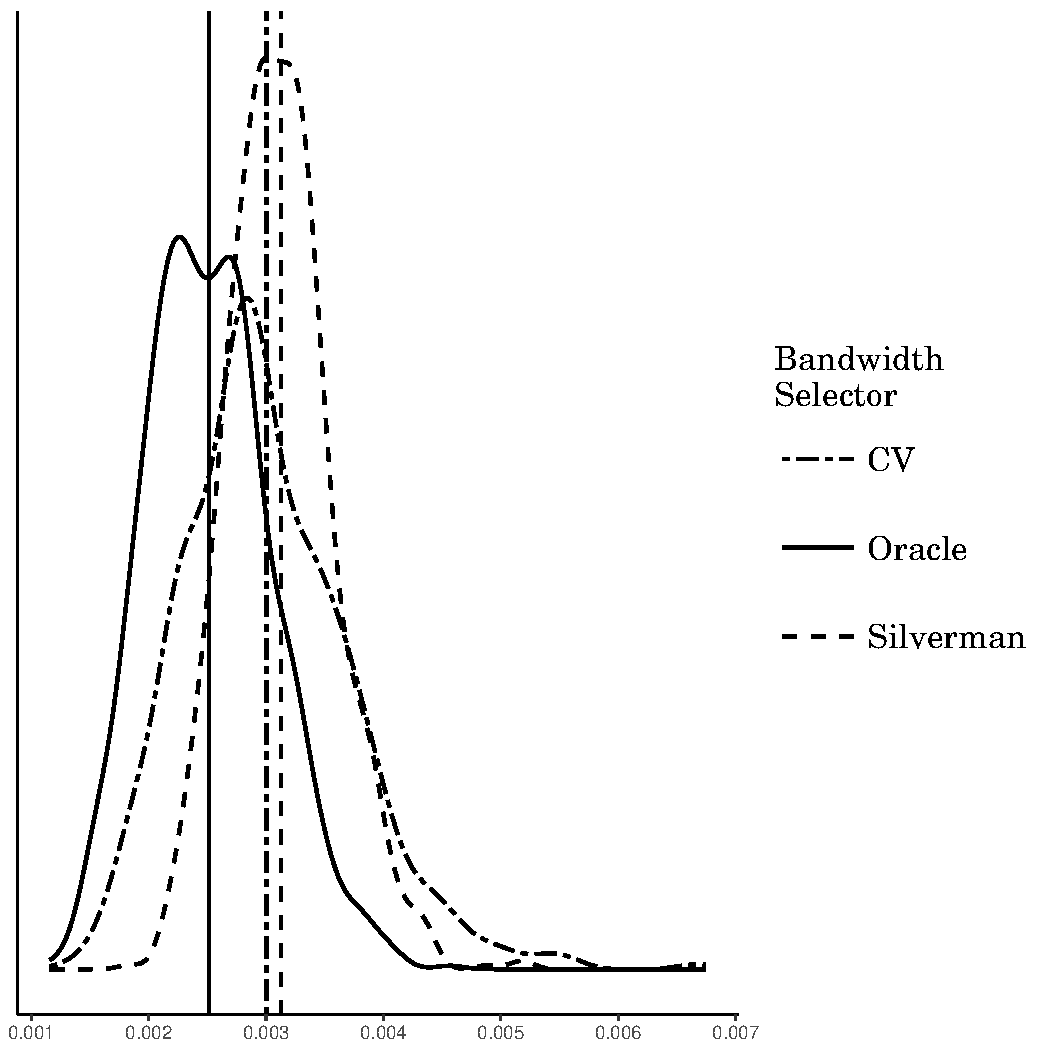
\includegraphics[width=\textwidth]{output/iae-histogram}
    \caption{Absolute IAE}
    \end{subfigure}
    \caption[IAE: uniform on uniform]{Integrated absolute error histogram for uniform intensity on a uniform population, 100 cases}
    \label{fig:iae:template}
\end{figure}

%%%%%%%%%%%%%%%%%%%%%%%%%%%%%%%%%%%%%%%%%%%%%%%%%
% Max error distribution - template
%%%%%%%%%%%%%%%%%%%%%%%%%%%%%%%%%%%%%%%%%%%%%%%%%
\begin{figure}[htbp]
    \centering
    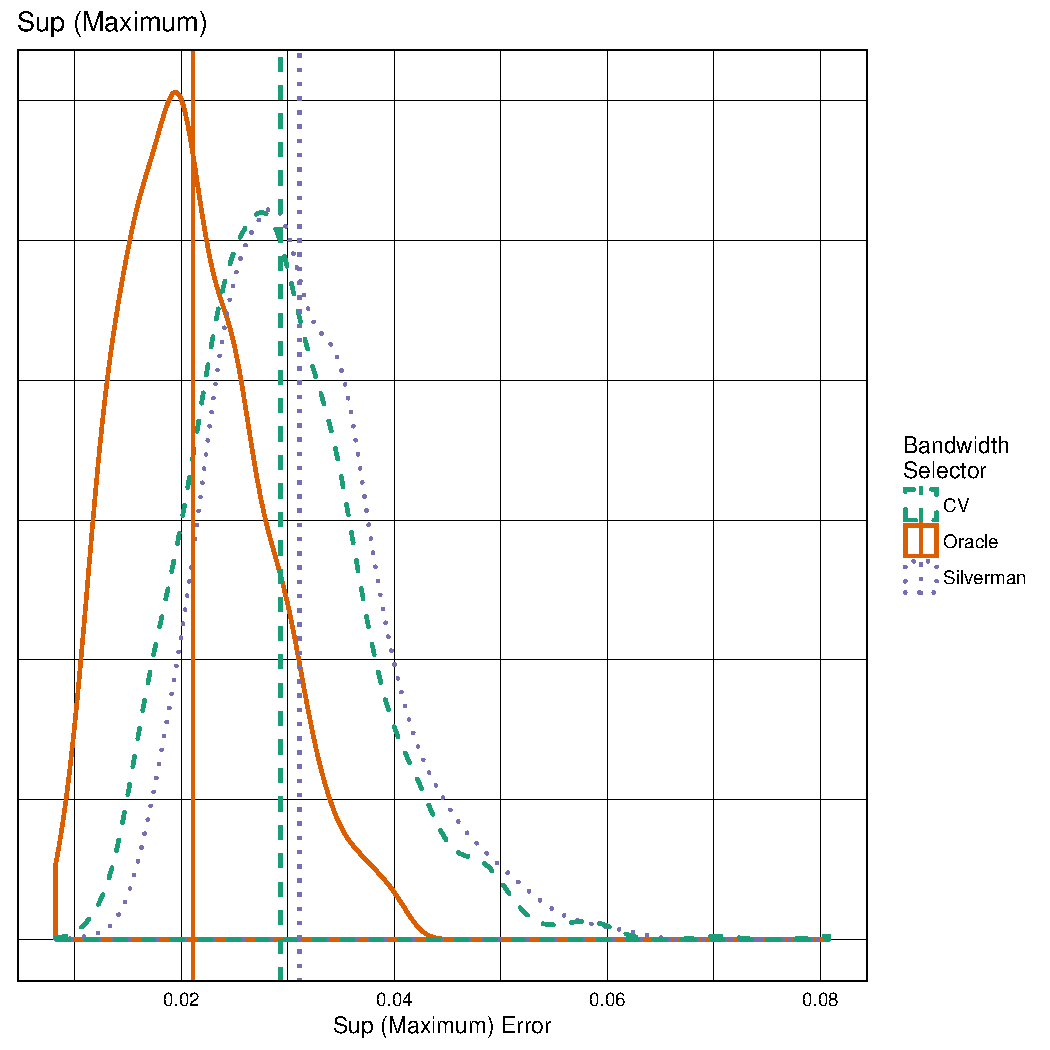
\includegraphics[width=0.45\textwidth]{output/maxerr-histogram}
    \caption[Maximum error: uniform on uniform]{Maximum error histogram for uniform intensity on a uniform population, 100 cases}
    \label{fig:maxerr:template}
\end{figure}

%%%%%%%%%%%%%%%%%%%%%%%%%%%%%%%%%%%%%%%%%%%%%%%%%
% Mean errors - template
%%%%%%%%%%%%%%%%%%%%%%%%%%%%%%%%%%%%%%%%%%%%%%%%%
\begin{table}[htbp]
\centering
% latex table generated in R 3.4.2 by xtable 1.8-2 package
% Sat Feb 17 16:44:44 2018
\begin{tabular}{lrrr}
  \hline
 & Oracle & Silverman & CV \\ 
  \hline
MISE & 0.000053 & 0.000083 & 0.000080 \\ 
  Relative MISE & 0.002028 & 0.003195 & 0.003047 \\ 
  Normalized MISE & 0.000026 & 0.000042 & 0.000040 \\ 
  MIAE & 0.003914 & 0.004863 & 0.004653 \\ 
  Relative MIAE & 0.024227 & 0.030102 & 0.028802 \\ 
  Max Error & 0.033855 & 0.049415 & 0.045884 \\ 
  Peak bias & -0.016050 & 0.010816 & -0.002953 \\ 
  Relative Peak bias & -0.099339 & 0.066949 & -0.018278 \\ 
  Peak drift & 0.223424 & 0.357624 & 0.284159 \\ 
  Relative Peak drift & 0.031918 & 0.051089 & 0.040594 \\ 
  Centroid bias & -0.017140 & -0.000902 & -0.013918 \\ 
  Relative Centroid bias & -0.106087 & -0.005583 & -0.086149 \\ 
  Centroid drift & 0.149249 & 0.159867 & 0.152694 \\ 
  Relative Centroid drift & 0.021321 & 0.022838 & 0.021813 \\ 
   \hline
\end{tabular}

\caption{Mean error rates for uniform population, uniform intensity of factor 100}
\label{tab:errors:template}
\end{table}

%%%%%%%%%%%%%%%%%%%%%%%%%%%%%%%%%%%%%%%%%%%%%%%%%
% Peaks - template
%%%%%%%%%%%%%%%%%%%%%%%%%%%%%%%%%%%%%%%%%%%%%%%%%
\begin{figure}[htbp]
    \centering
    \begin{subfigure}[b]{0.45\textwidth}
    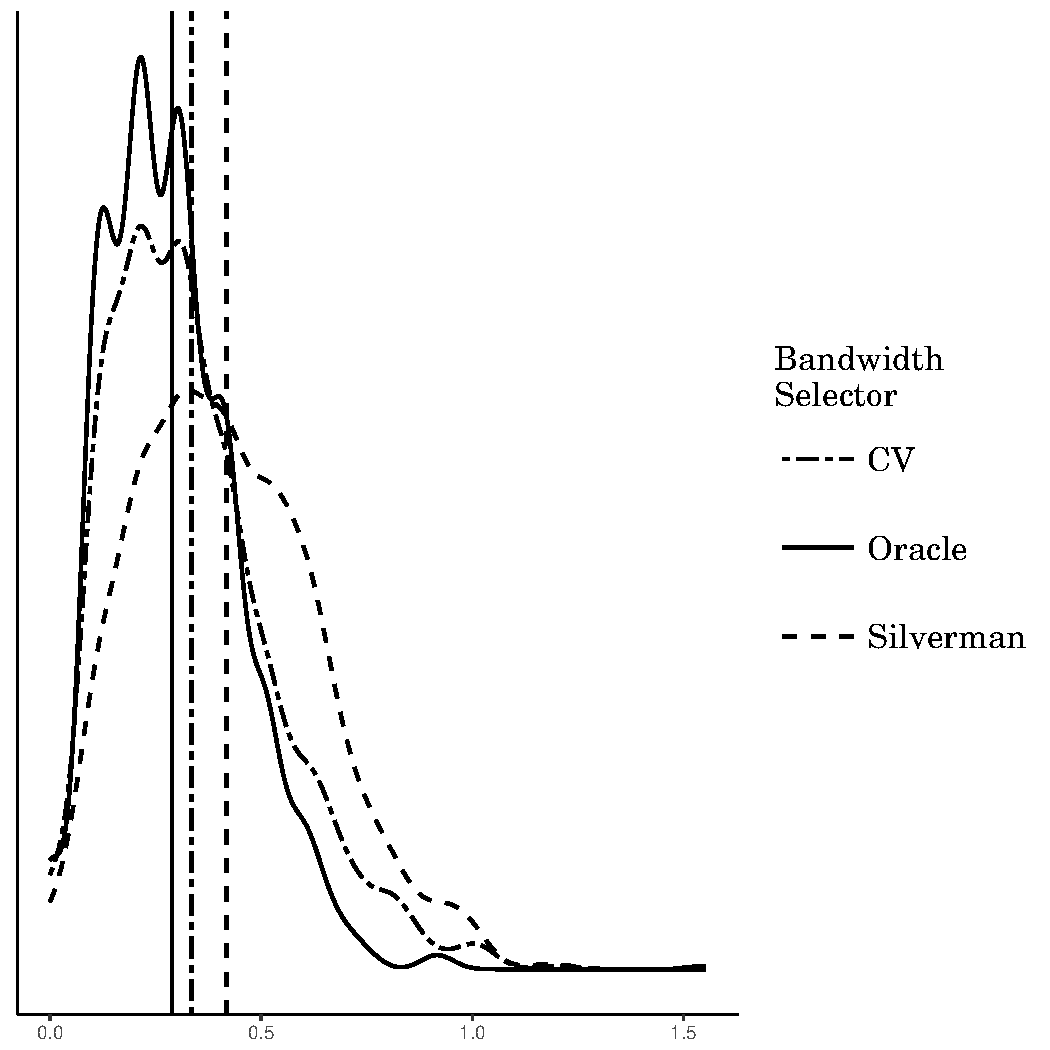
\includegraphics[width=\textwidth]{output/peak-dist-histogram}
    \caption{Peak distance from truth}
    \end{subfigure}
    \begin{subfigure}[b]{0.45\textwidth}
    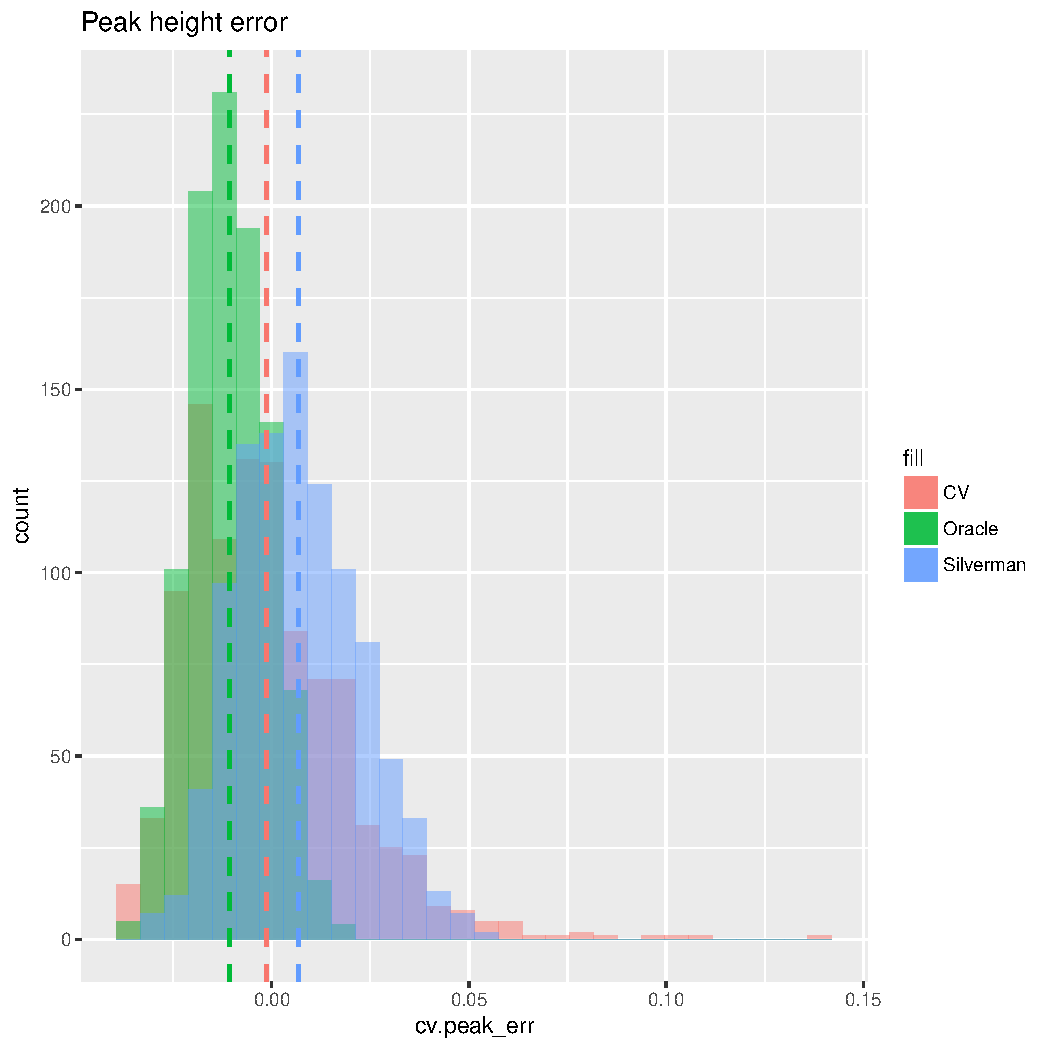
\includegraphics[width=\textwidth]{output/peak-height-histogram}
    \caption{Peak heights}
    \end{subfigure}
    \caption[Peaks: uniform on uniform]{Peak distance from truth and height histograms for uniform intensity on a uniform population, 100 cases}
    \label{fig:iae:template}
\end{figure}

%%%%%%%%%%%%%%%%%%%%%%%%%%%%%%%%%%%%%%%%%%%%%%%%%
% Centroids - template
%%%%%%%%%%%%%%%%%%%%%%%%%%%%%%%%%%%%%%%%%%%%%%%%%
\begin{figure}[htbp]
    \centering
    \begin{subfigure}[b]{0.45\textwidth}
    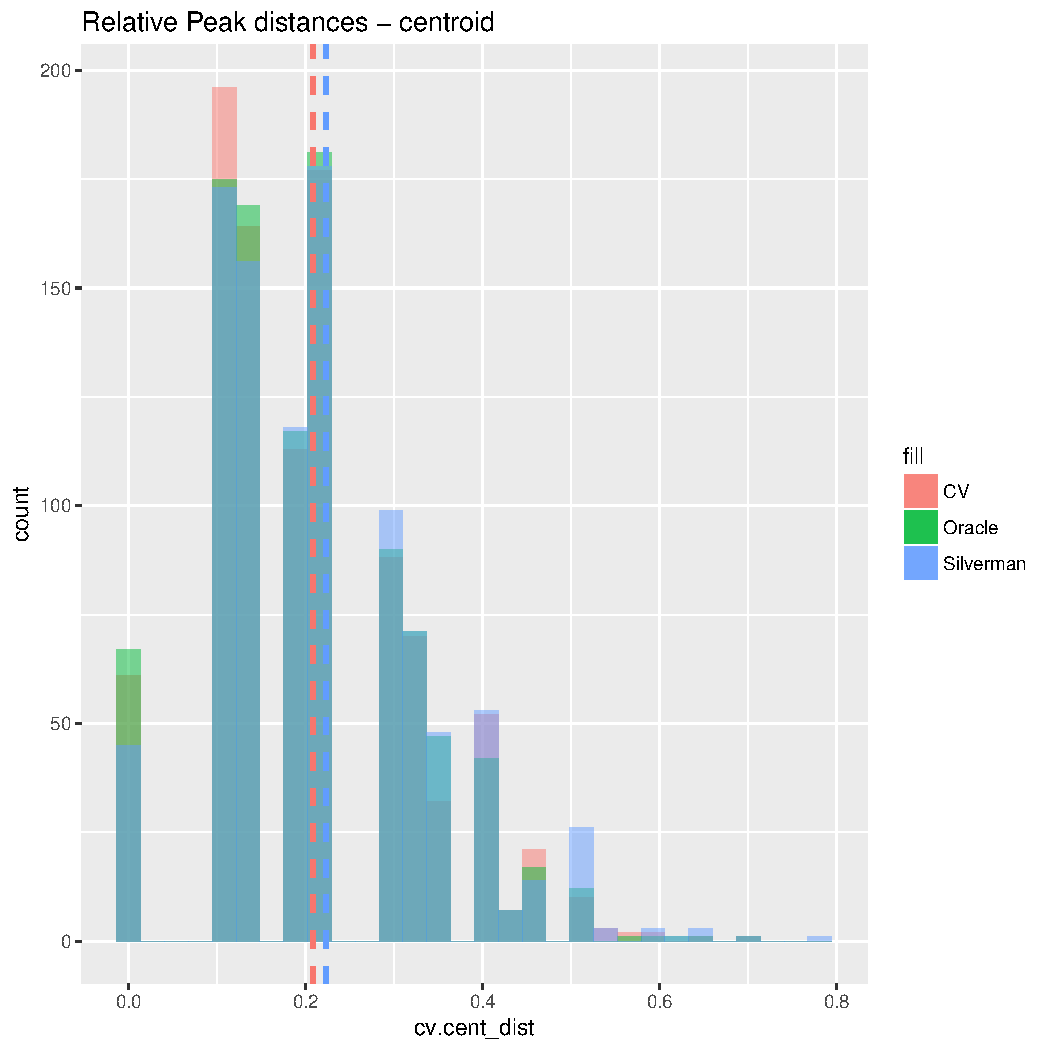
\includegraphics[width=\textwidth]{output/centroid-dist-histogram}
    \caption{Centroid peak distance from truth}
    \end{subfigure}
    \begin{subfigure}[b]{0.45\textwidth}
    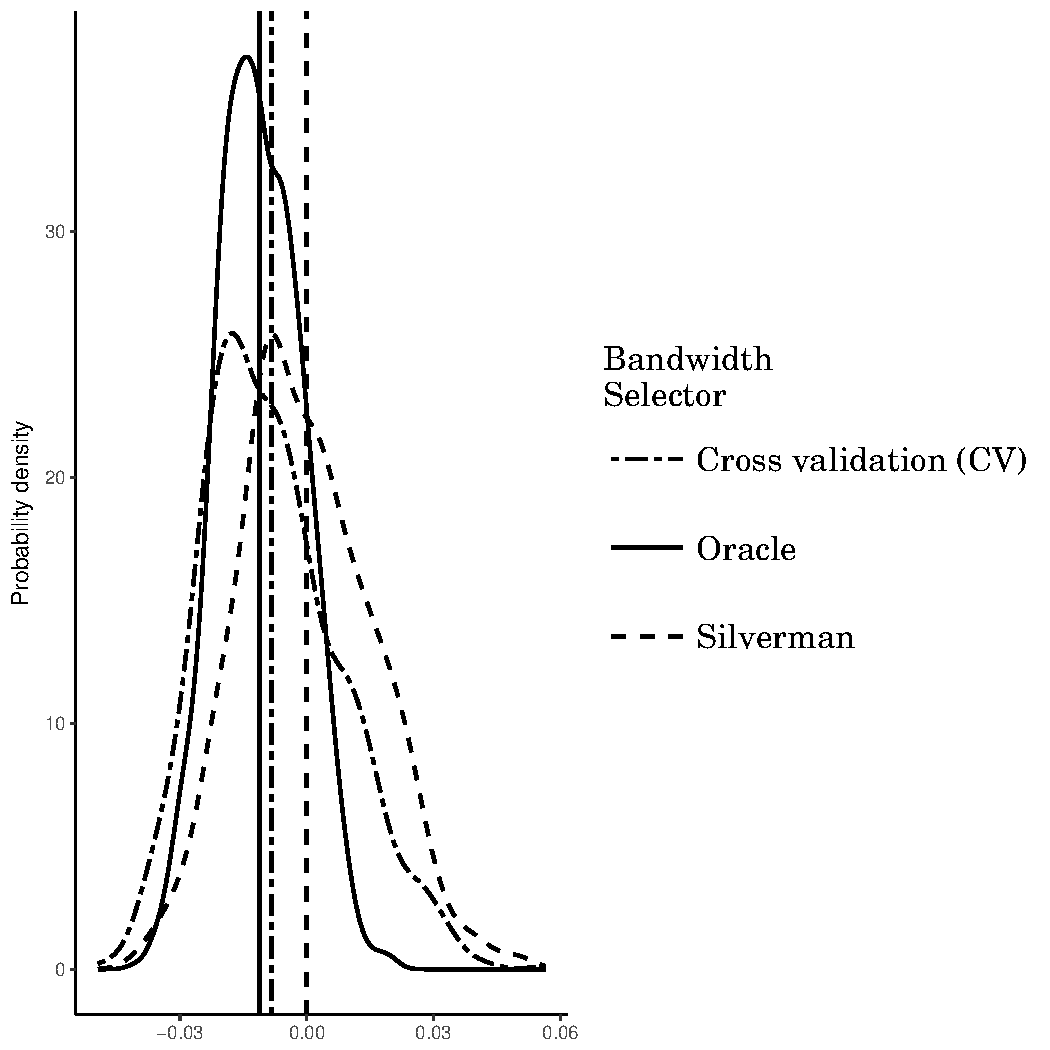
\includegraphics[width=\textwidth]{output/centroid-height-histogram}
    \caption{Centroid peak heights}
    \end{subfigure}
    \caption[Centroids: uniform on uniform]{Centroid peak distance from truth and height histograms for uniform intensity on a uniform population, 100 cases}
    \label{fig:iae:template}
\end{figure}

%%%%%%%%%%%%%%%%%%%%%%%%%%%%%%%%%%%%%%%%%%%%%%%%%
% Bandwidths - template
%%%%%%%%%%%%%%%%%%%%%%%%%%%%%%%%%%%%%%%%%%%%%%%%%
\begin{figure}[htbp]
    \centering
    \begin{subfigure}[b]{0.45\textwidth}
    \includegraphics[width=\textwidth]{output/bandwidths-x1}
    \caption{CV Bandwidths - \(X_1\)}
    \end{subfigure}
    \begin{subfigure}[b]{0.45\textwidth}
    \includegraphics[width=\textwidth]{output/bandwidths-x2}
    \caption{CV Bandwidths - \(X_2\)}
    \end{subfigure}

    \begin{subfigure}[b]{0.45\textwidth}
    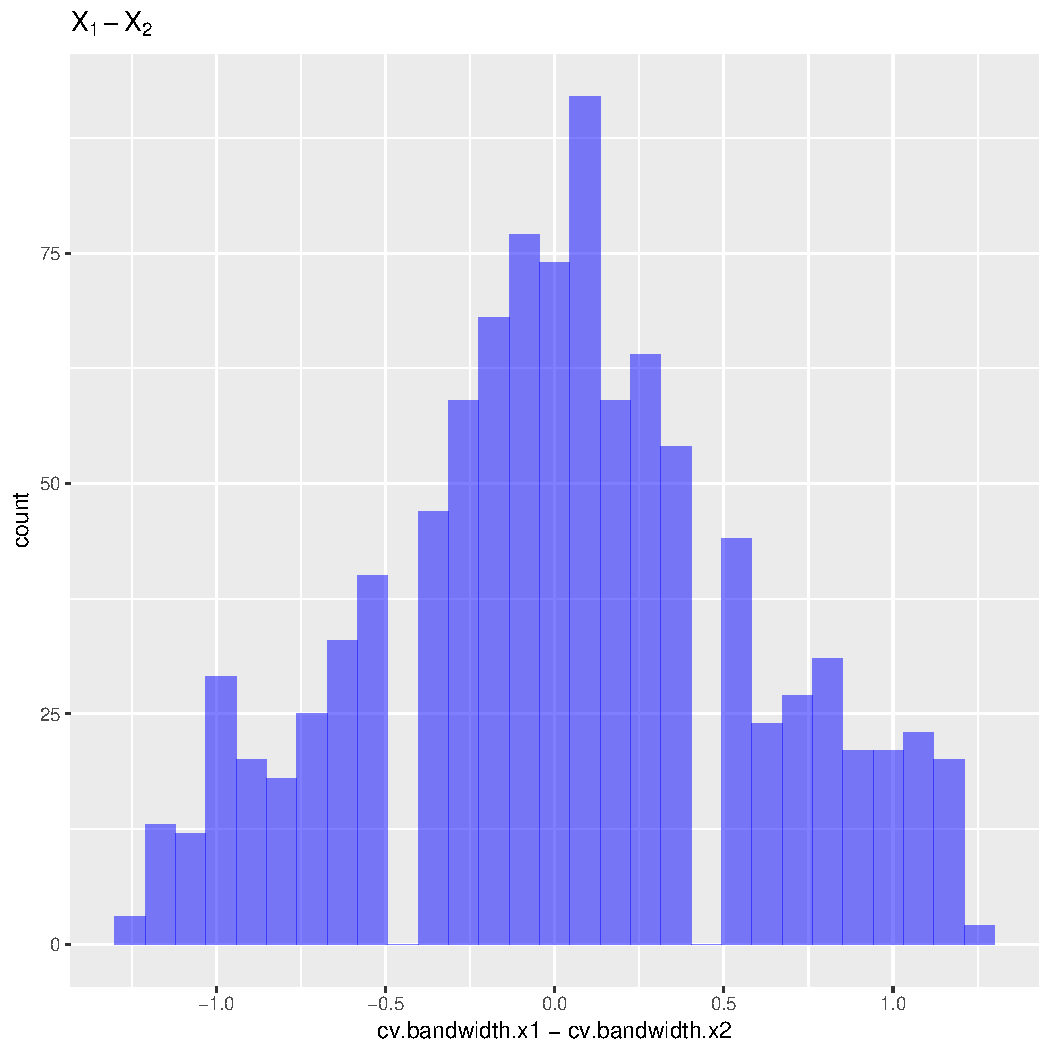
\includegraphics[width=\textwidth]{output/bandwidths-difference}
    \caption{Difference between \(X_1\) and \(X_2\) bandwidths}
    \end{subfigure}
    \begin{subfigure}[b]{0.45\textwidth}
    \includegraphics[width=\textwidth]{output/bandwidths-silverman}
    \caption{Silverman Bandwidths}
    \end{subfigure}
    \caption[Bandwidths: uniform on uniform]{CV bandwidths: \(X_1\), \(X_2\) and difference and Silverman bandwidth
        histograms for uniform intensity on a uniform population, 100 cases}
    \label{fig:iae:template}
\end{figure}


%%%%%%%%%%%%%%%%%%%%%%%%%%%%%%%%%%%%%%%%%%%%%%%%%
%%
%% Uniform risk on uniform population section
%%
%%%%%%%%%%%%%%%%%%%%%%%%%%%%%%%%%%%%%%%%%%%%%%%%%
\section{Uniform risk on a uniform population}
\label{sec:results:unif_100_unif}

%%%%%%%%%%%%%%%%%%%%%%%%%%%%%%%%%%%%%%%%%%%%%%%%%
% Parameter table - template
%%%%%%%%%%%%%%%%%%%%%%%%%%%%%%%%%%%%%%%%%%%%%%%%%
\begin{table}[htbp]
\centering
\begin{tabular}{ll}
\hline
Parameter & Value \\
\hline
Population size & 10,000 \\
Population decay rate & uniform \\
Incident risk factor & 100 \\
Incident decay rate & uniform \\
Incident center & -- \\
\hline
\end{tabular}
\caption{Parameters used in uniform risk on a uniform population}
\label{tab:params:unif_100_unif}
\end{table}

In this section, we describe the results of 1,000 simulations conducted for a population of 10,000 points,
distributed uniformly throughout the study area.
\autoref{fig:cases:unif_100_unif} shows the true uniform intensity function,
together with three estimated intensity functions of a single simulation,
computed using three bandwidths: the oracle bandwidth, the Silverman rule of thumb bandwidth,
and the cross-validation bandwidth.

\begin{figure}[htbp]
    \centering
    \begin{subfigure}[t]{0.45\textwidth}
    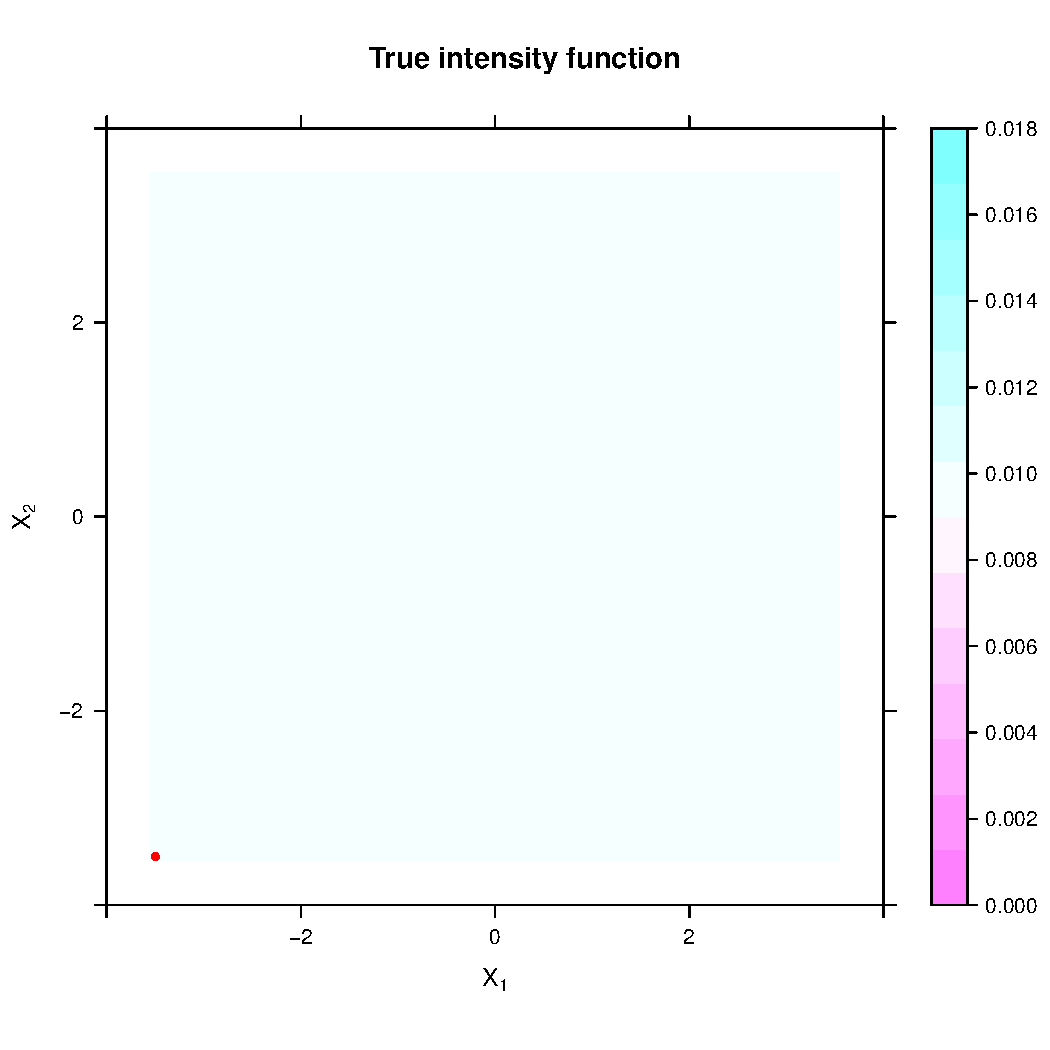
\includegraphics[width=\textwidth]{results/unif_100_unif/output/true_intensity_heatmap}
    \caption{True intensity}
    \end{subfigure}%
    \begin{subfigure}[t]{0.45\textwidth}
    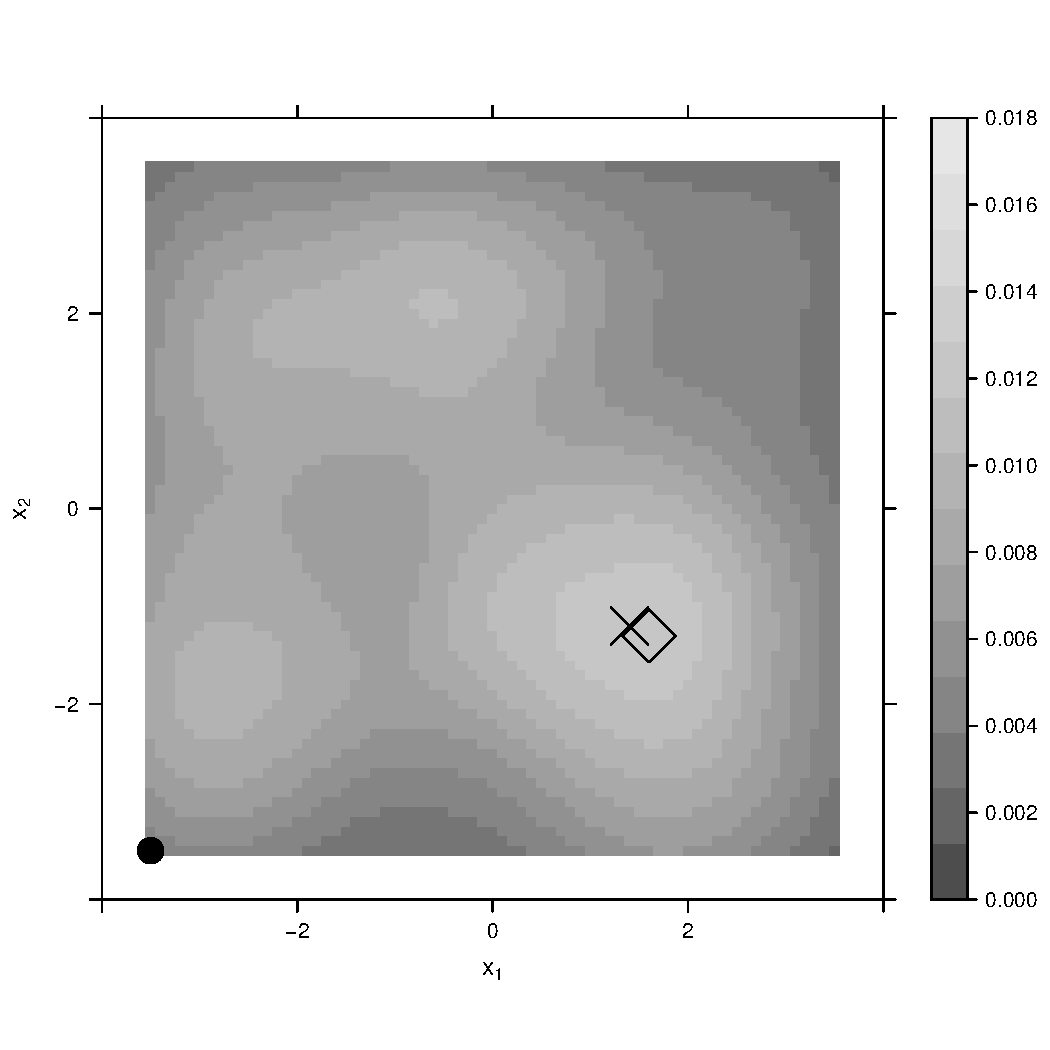
\includegraphics[width=\textwidth]{results/unif_100_unif/output/oracle_intensity_heatmap}
    \caption{Oracle bandwidth estimate}
    \end{subfigure}


    \begin{subfigure}[b]{0.45\textwidth}
    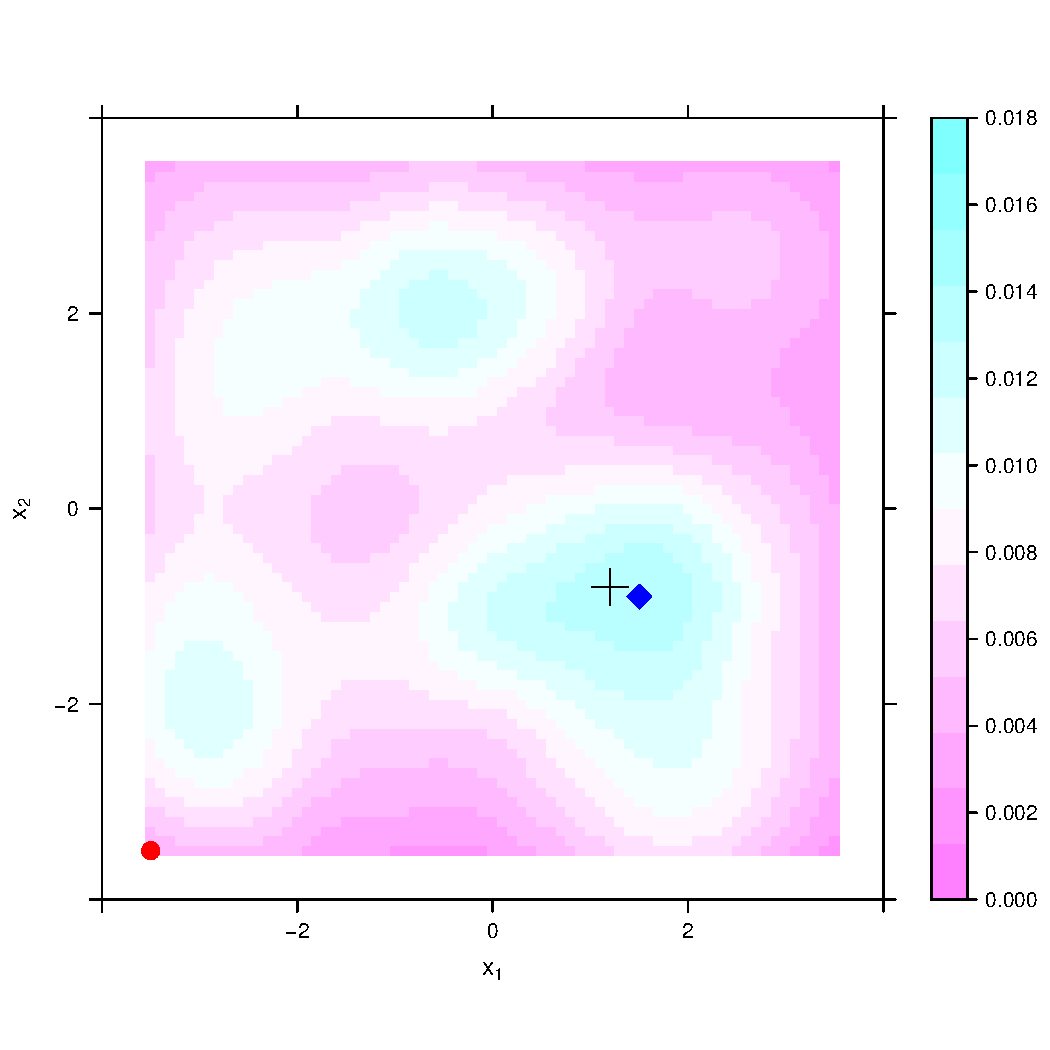
\includegraphics[width=\textwidth]{results/unif_100_unif/output/silverman_intensity_heatmap}
    \caption{Silverman bandwidth estimate}
    \end{subfigure}%
    \begin{subfigure}[b]{0.45\textwidth}
    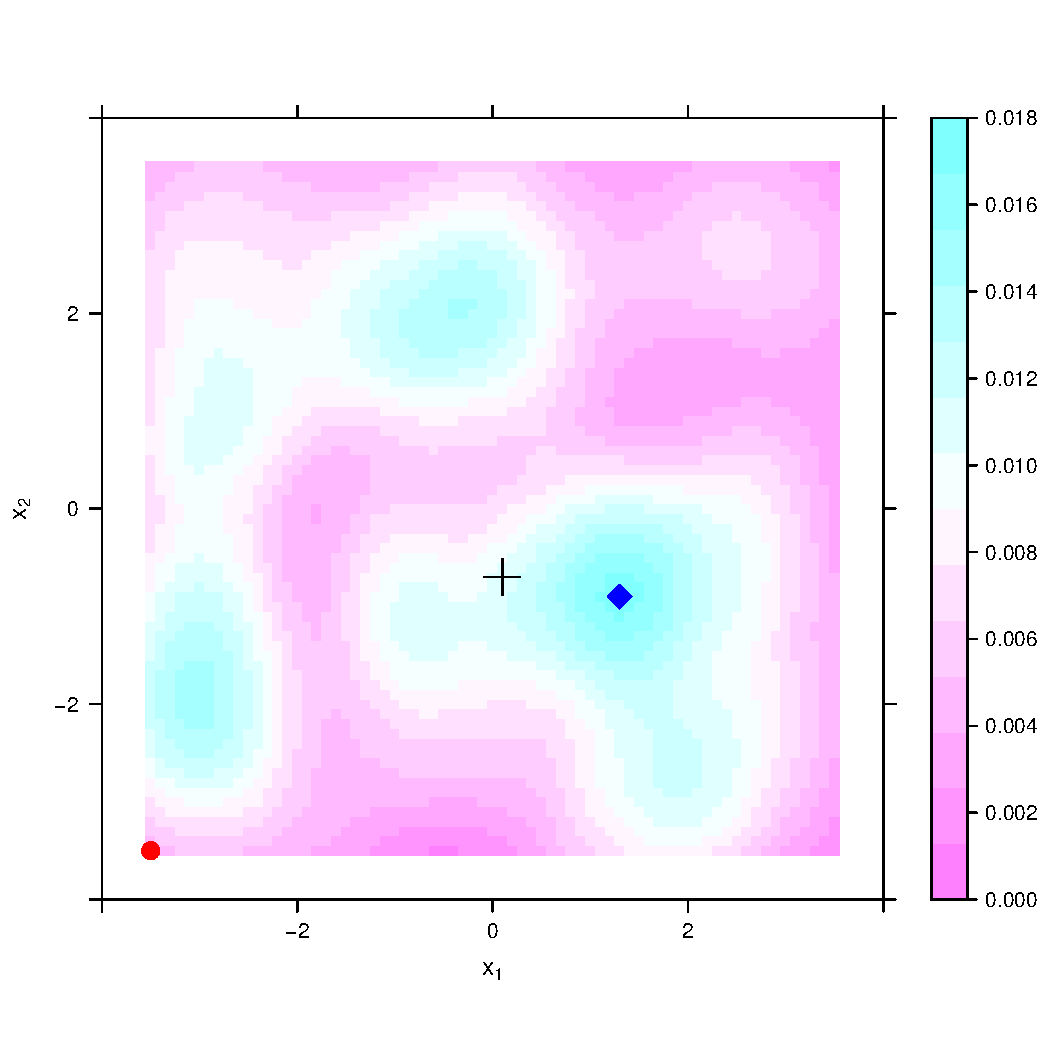
\includegraphics[width=\textwidth]{results/unif_100_unif/output/CV_intensity_heatmap}
    \caption{Cross-validation bandwidth estimate}
    \end{subfigure}
    \caption{Example cases: uniform intensity on uniform population, 100 cases}
    \label{fig:cases:unif_100_unif}
\end{figure}

\begin{table}[htbp]
\centering
% latex table generated in R 3.4.0 by xtable 1.8-2 package
% Sat Aug  5 20:02:24 2017
\begin{tabular}{lrrr}
  \hline
 & Oracle & Silverman & CV \\ 
  \hline
MISE & 0.000012 & 0.000013 & 0.000013 \\ 
  Relative MISE & 0.117027 & 0.127810 & 0.127803 \\ 
  MIAE & 0.002801 & 0.002922 & 0.002922 \\ 
  Relative MIAE & 0.280127 & 0.292163 & 0.292156 \\ 
  Max Error & 0.008572 & 0.009040 & 0.009040 \\ 
  Peak bias & 0.003361 & 0.005616 & 0.005615 \\ 
  Relative Peak bias & 0.336092 & 0.561583 & 0.561492 \\ 
  Peak drift & 5.163912 & 5.190480 & 5.190393 \\ 
  Relative Peak drift & 0.737702 & 0.741497 & 0.741485 \\ 
  Centroid bias & 0.002819 & 0.003733 & 0.003733 \\ 
  Relative Centroid bias & 0.281890 & 0.373345 & 0.373340 \\ 
  Centroid drift & 5.093476 & 5.086491 & 5.086412 \\ 
  Relative Centroid drift & 0.727639 & 0.726642 & 0.726630 \\ 
   \hline
\end{tabular}

\caption{Mean error rates for uniform population, uniform intensity of factor 100}
\label{tab:errors:unif_100_unif}
\end{table}

\autoref{tab:errors:unif_100_unif} lists the mean error rates obtained for a uniform intensity with factor of 100,
over a uniform population of 10,000.
The columns represent the errors observed by using the three different methods for computing the smoothing bandwidth:
the Oracle, the Silverman rule of thumb, and least-squares cross validation.
Each row represents a different measure of error.
Relative MISE is the mean integrated relative squared error,
where the relative squared error is computed in the following manner:
\[ \mbox{RSE}(x) = \left(\frac{\hat{f}(x)-f(x)}{f(x)}\right)^2 .\]
More generally, the relative error at a point \(x\) is computed as
\[ \mbox{RE}(x) =  \frac{\hat{f}(x)-f(x)}{f(x)} .\]
The next row is the mean integrated absolute error (MIAE),
which is followed by Relative MIAE which is computed analogously to Relative MISE.
This is followed by the Maximum error, which is the greatest absolute error over the study area.
Complete results can be found in \autoref{tab:mean_error_rates:unif_100_unif} in \autoref{chp:results_tables}.

The error measures mentioned above each compare the closeness of the estimated intensity function to the true funcition.
The following error measures, on the other hand, relate the closeness of the \textit{peak} of the estimate to the true peak.
The \textit{peak bias} is the average difference between the computed and true maxima,
that is the empirical expectation of \(\max{\{\hat{f}(x)\}} - \max{\{f(x)\}}\).
The Relative peak bias is peak bias expressed relative to the true maximum.
The \textit{peak drift} is the Euclidean distance between the estimated peak and the true peak.
The Relative peak drift is the peak drift, expressed relative to the width of the study area.

The next four measures, \textit{centroid bias} and \textit{drift}, and the relative versions of them, are analogous to the peak error measures.
However, instead of comparing the true peak to the peak of the estimate, they compare it to the location and value of the estimate, calculated at the centroid of the top five percent of the estimated function.

\begin{figure}[htbp]
    \centering
    \begin{subfigure}[b]{0.45\textwidth}
    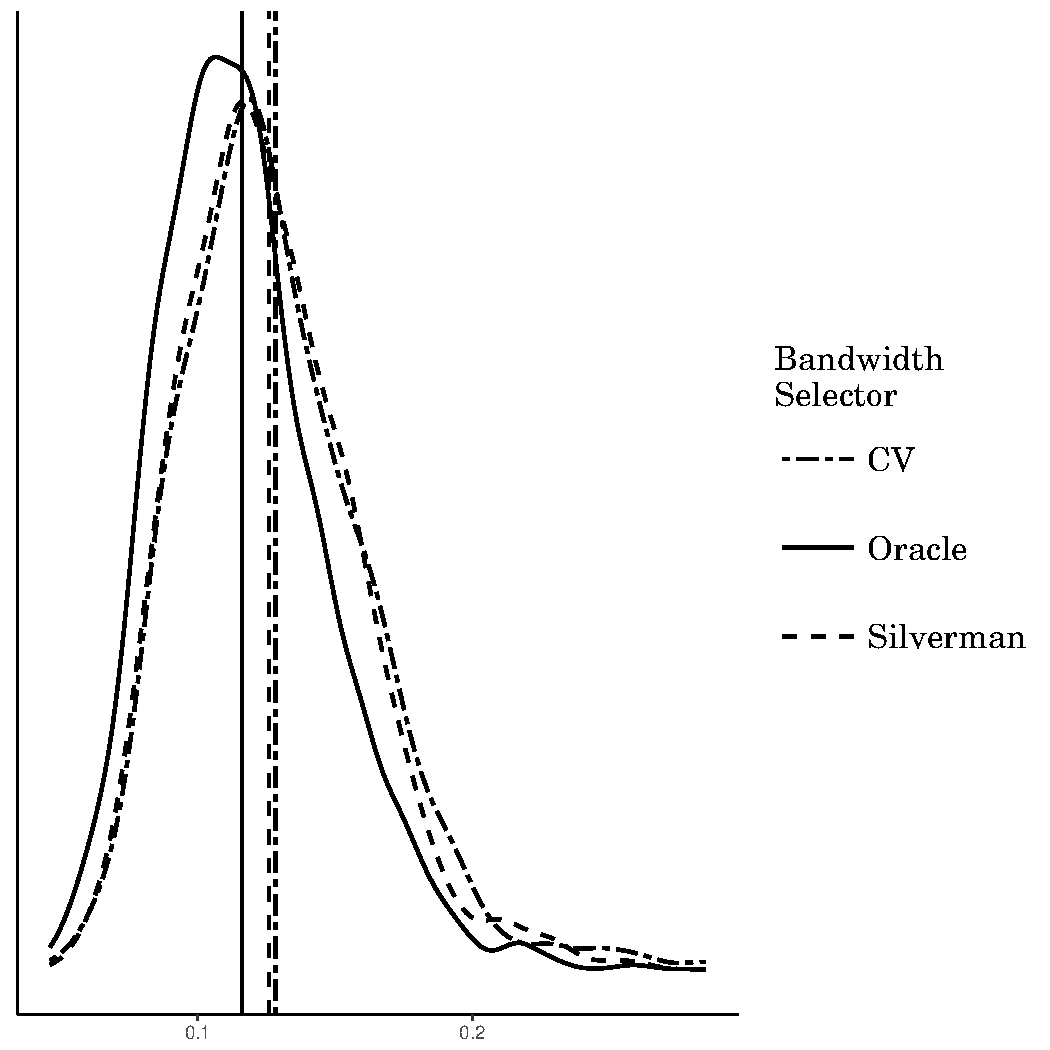
\includegraphics[width=\textwidth]{results/unif_100_unif/output/ise-relative-histogram}
    \caption{Relative ISE}
    \end{subfigure}
    \begin{subfigure}[b]{0.45\textwidth}
    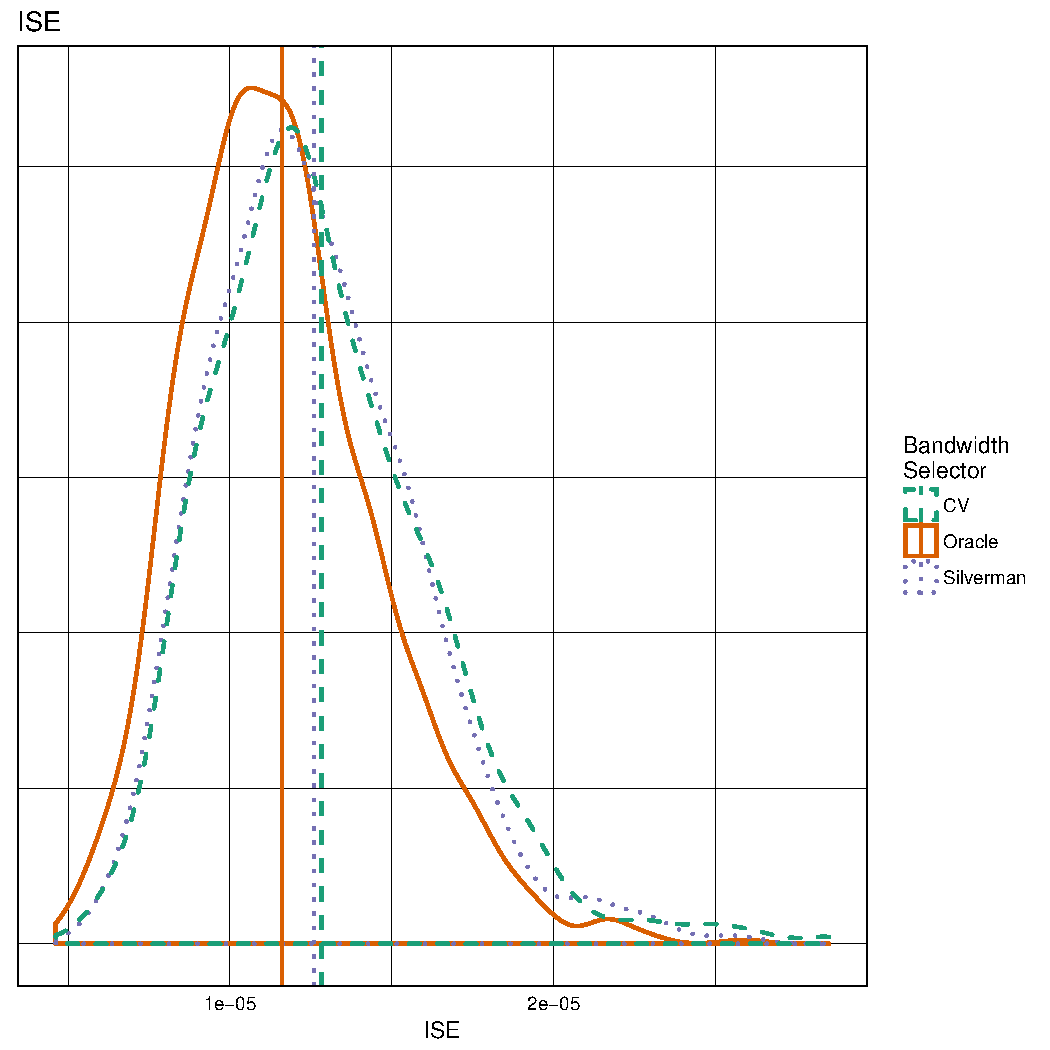
\includegraphics[width=\textwidth]{results/unif_100_unif/output/ise-histogram}
    \caption{Absolute ISE}
    \end{subfigure}
    \caption[ISE: uniform on uniform]{Integrated squared error histogram for uniform intensity on a uniform population, 100 cases}
    \label{fig:ise:unif_100_unif}
\end{figure}

\autoref{fig:ise:unif_100_unif} shows the empirical distribution of the MISE and RMISE for the uniform intensity on uniform population.
The similarity of the distributions for the Oracle, Silverman, and Cross-validation bandwidths
reflects the relative ease with which the DKD can estimate a flat intensity function.

\begin{figure}[htbp]
    \centering
    \begin{subfigure}[b]{0.3\textwidth}
    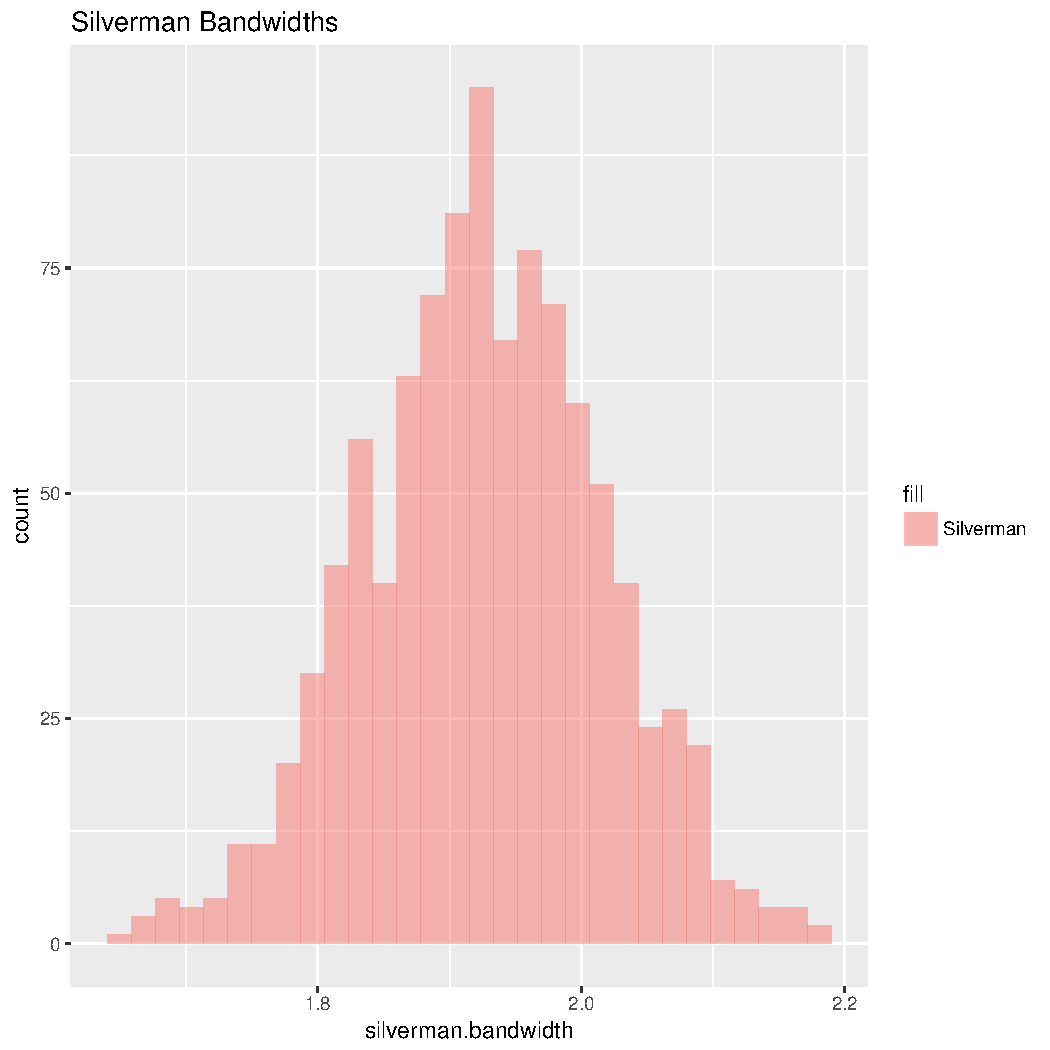
\includegraphics[width=\textwidth]{results/unif_100_unif/output/bandwidths-silverman}
    \caption{Silverman}
    \label{fig:bandwidths_x1:unif_100_unif:s}
    \end{subfigure}
    \begin{subfigure}[b]{0.3\textwidth}
    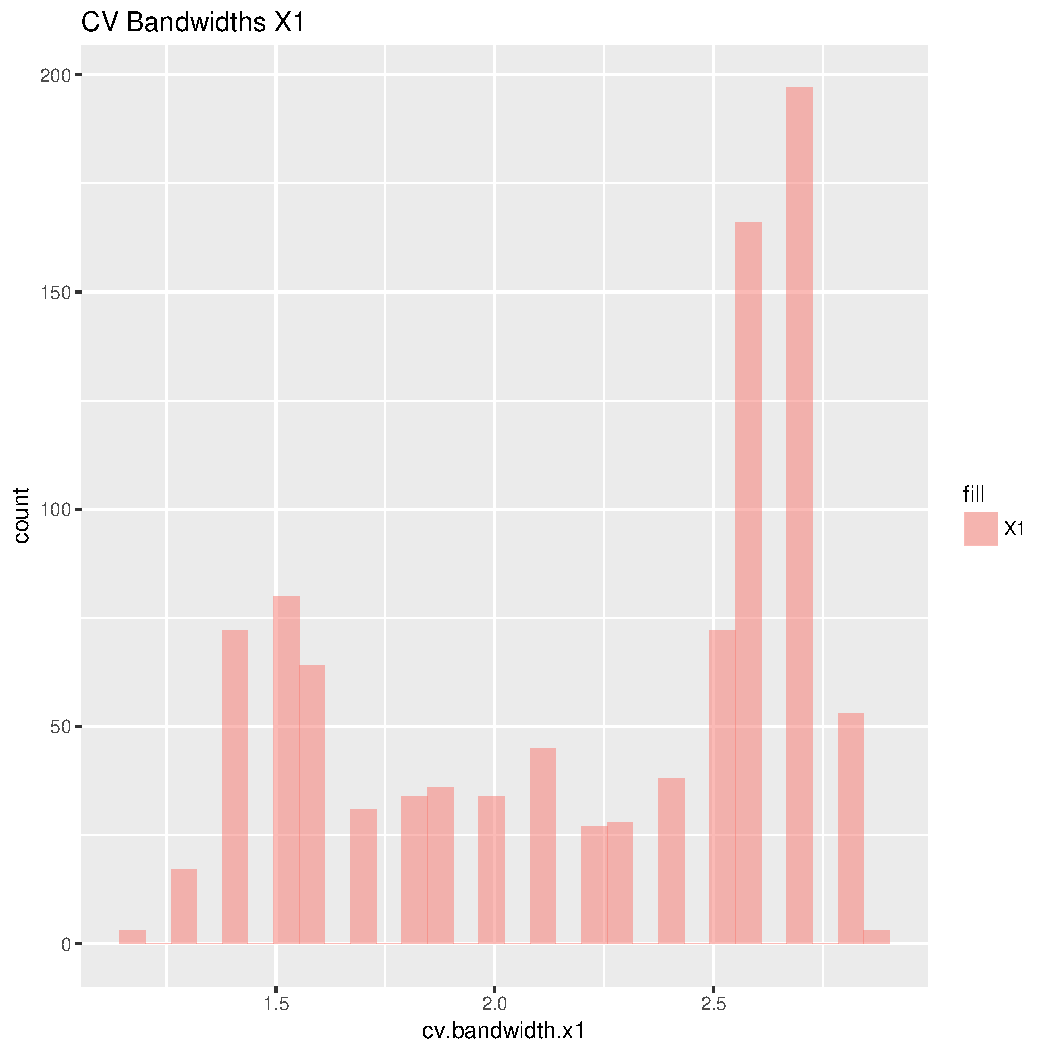
\includegraphics[width=\textwidth]{results/unif_100_unif/output/bandwidths-x1}
    \caption{Cross-validation, \(X_1\)}
    \label{fig:bandwidths_x1:unif_100_unif:x1}
    \end{subfigure}
    \begin{subfigure}[b]{0.3\textwidth}
    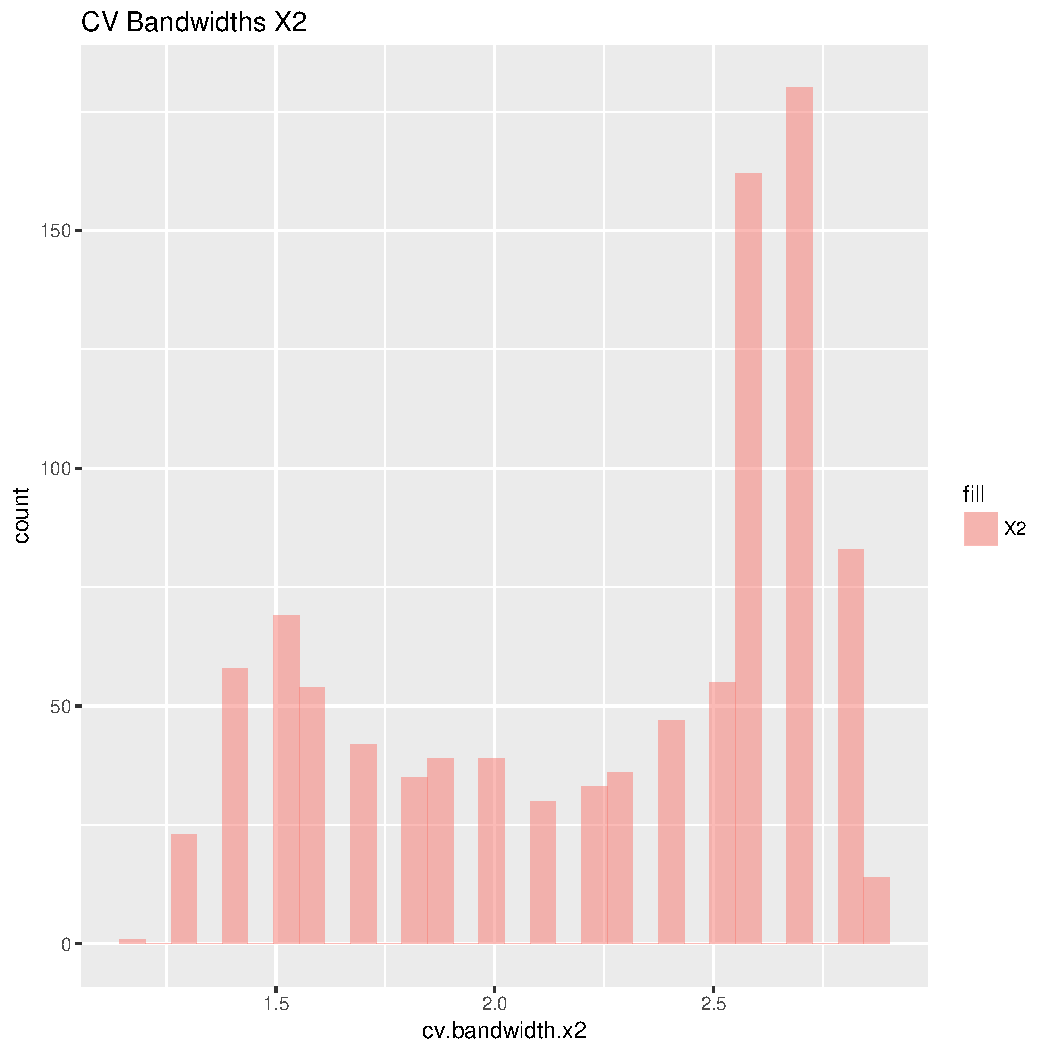
\includegraphics[width=\textwidth]{results/unif_100_unif/output/bandwidths-x2}
    \caption{Cross-validation, \(X_2\)}
    \label{fig:bandwidths_x1:unif_100_unif:x2}
    \end{subfigure}
    \caption{Bandwidth histograms for 100 incidents (uniform) from population of 10,000}
\end{figure}


%%
%% Section
\section{Varying the number of incidents}
\label{sec:results:unif_NCases_1h}

%%%%%%%%%%%%%%%%%%%%%%%%%%%%%
% Parameter table
%%%%%%%%%%%%%%%%%%%%%%%%%%%%%
\begin{table}[htbp]
\centering
\begin{tabular}{ll}
\hline
Parameter & Value \\
\hline
Population size & 10,000 \\
Population decay rate & uniform \\
Incident risk factor & 50, 100, 200, 500, 1000 \\
Incident decay rate & 1.0 \\
Incident center & (0,0) \\
\hline
\end{tabular}
\caption{Parameters used for varying the number of incidents}
\label{tab:params:unif_NCases_1h}
\end{table}

In this section we examine and compare the results of experiments where the number of incidents is varied, while keeping the population size constant at 10,000, distributed uniformly throughout the study area.
The expected incident sizes used in the experiments in this section were 50, 100, 200, 500, and 1,000.
The full set of error measures for these cases can be found in \autoref{tab:mean_error_rates:unif_50_1.0_1h}, \autoref{tab:mean_error_rates:unif_100_1.0_1h}, \autoref{tab:mean_error_rates:unif_200_1.0_1h}, \autoref{tab:mean_error_rates:unif_500_1.0_1h}, and \autoref{tab:mean_error_rates:unif_100_1.0_1h} in \autoref{chp:results_tables}.


\begin{figure}[htbp]
    \centering
    \begin{subfigure}{0.45\textwidth}
    \includegraphics[width=\textwidth]{results/unif_100_1.0_1h/output/population_and_incidents_scatter}
    \caption{100 incidents}
    \end{subfigure}
    \begin{subfigure}{0.45\textwidth}
    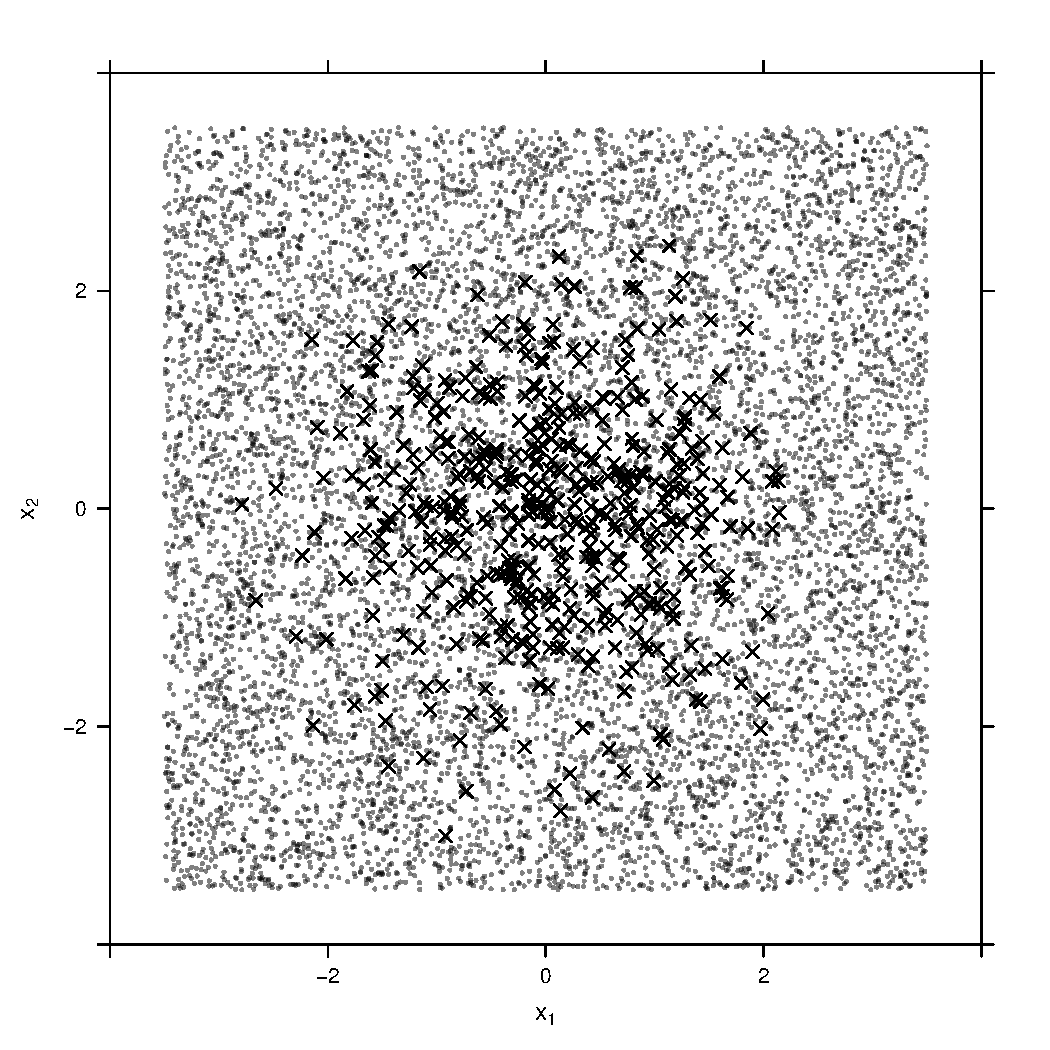
\includegraphics[width=\textwidth]{results/unif_500_1.0_1h/output/population_and_incidents_scatter}
    \caption{500 incidents}
    \end{subfigure}
    \caption{A single realization of different sizes from a single-peak risk on a uniform population}
    \label{fig:one_sample:unif_NCases_1h}
\end{figure}

\begin{figure}[htbp]
    \centering
    \begin{subfigure}[b]{0.3\textwidth}
    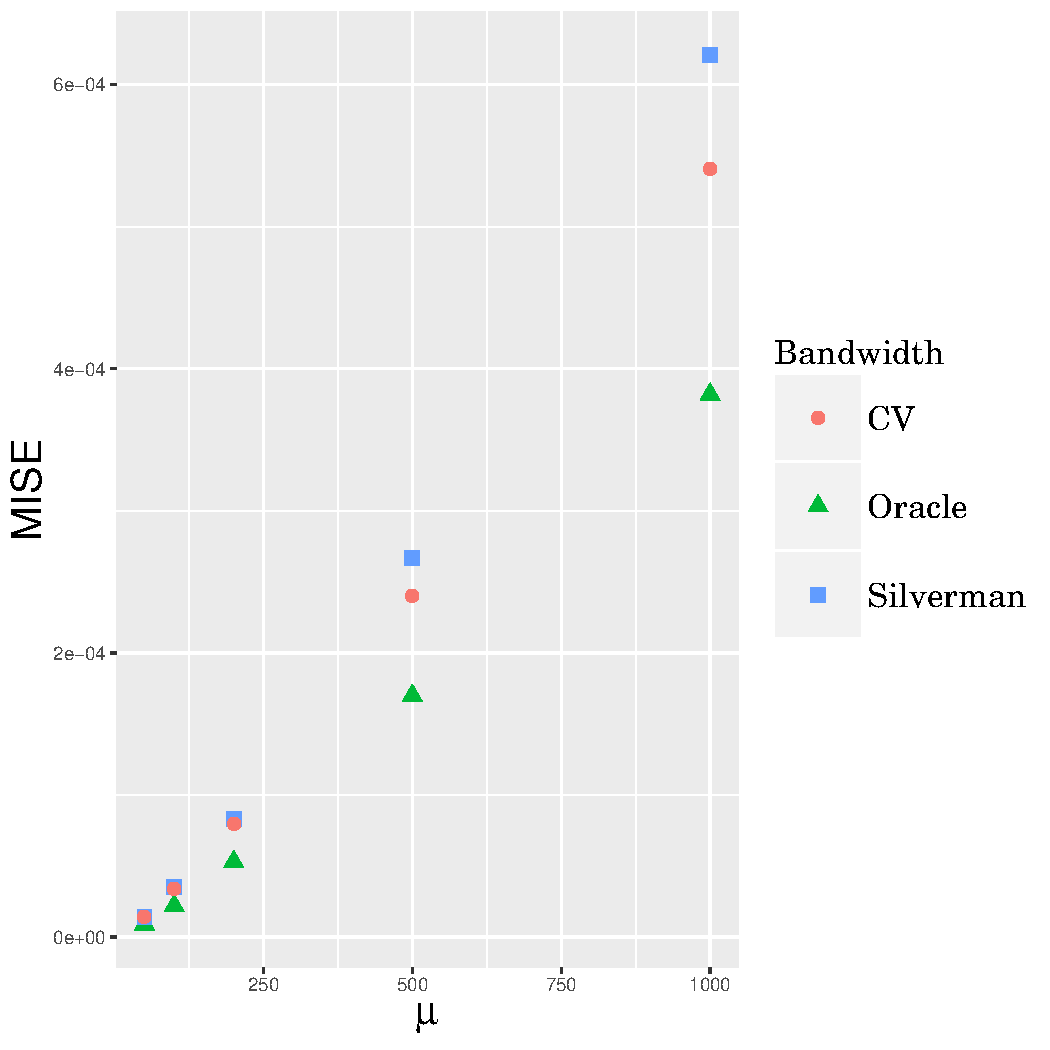
\includegraphics[width=\textwidth]{results/by_num_cases/MISE-vs-cases}
    \caption{MISE}
    \label{fig:ise:unif_NCases_1h:a}
    \end{subfigure}
    \begin{subfigure}[b]{0.3\textwidth}
    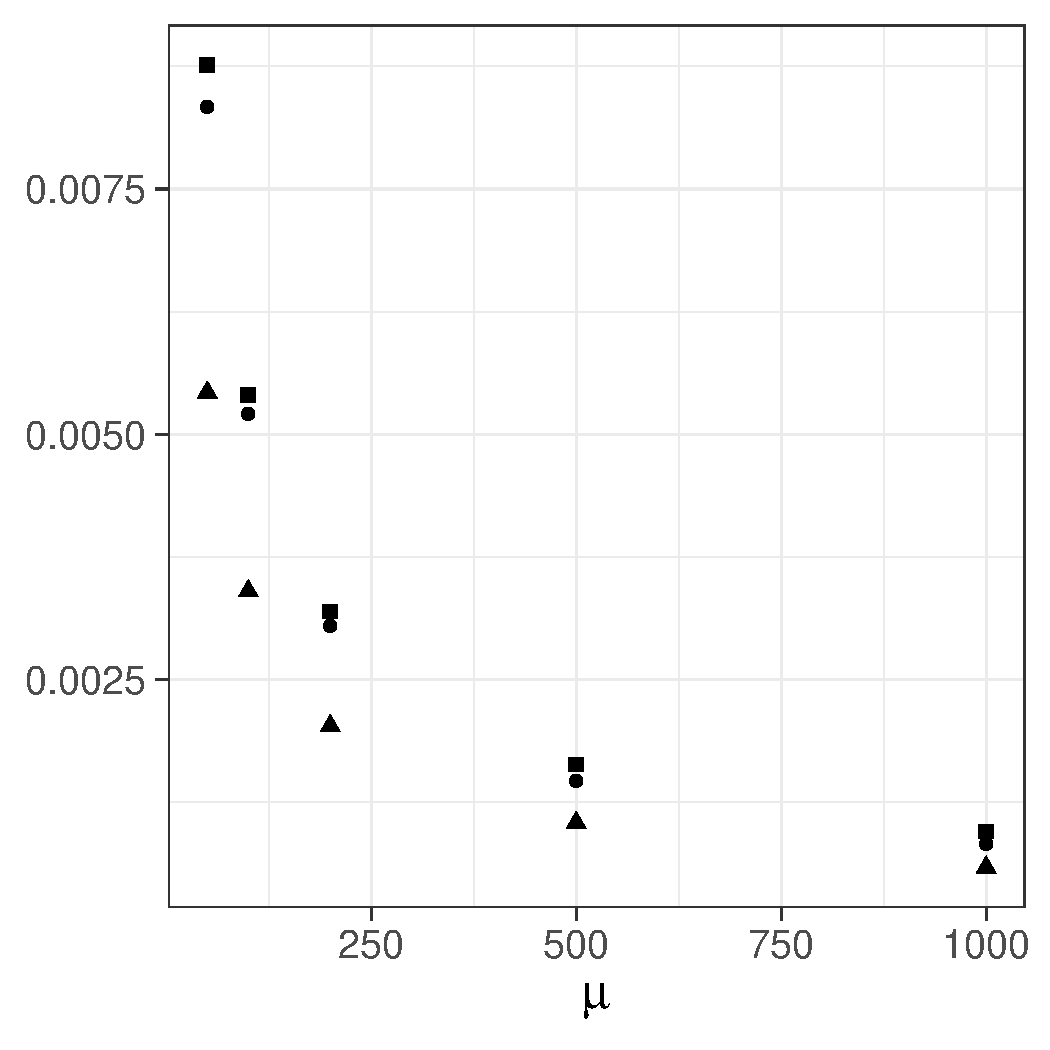
\includegraphics[width=\textwidth]{results/by_num_cases/RMISE-vs-cases}
    \caption{Relative MISE}
    \label{fig:ise:unif_NCases_1h:b}
    \end{subfigure}
    \begin{subfigure}[b]{0.3\textwidth}
    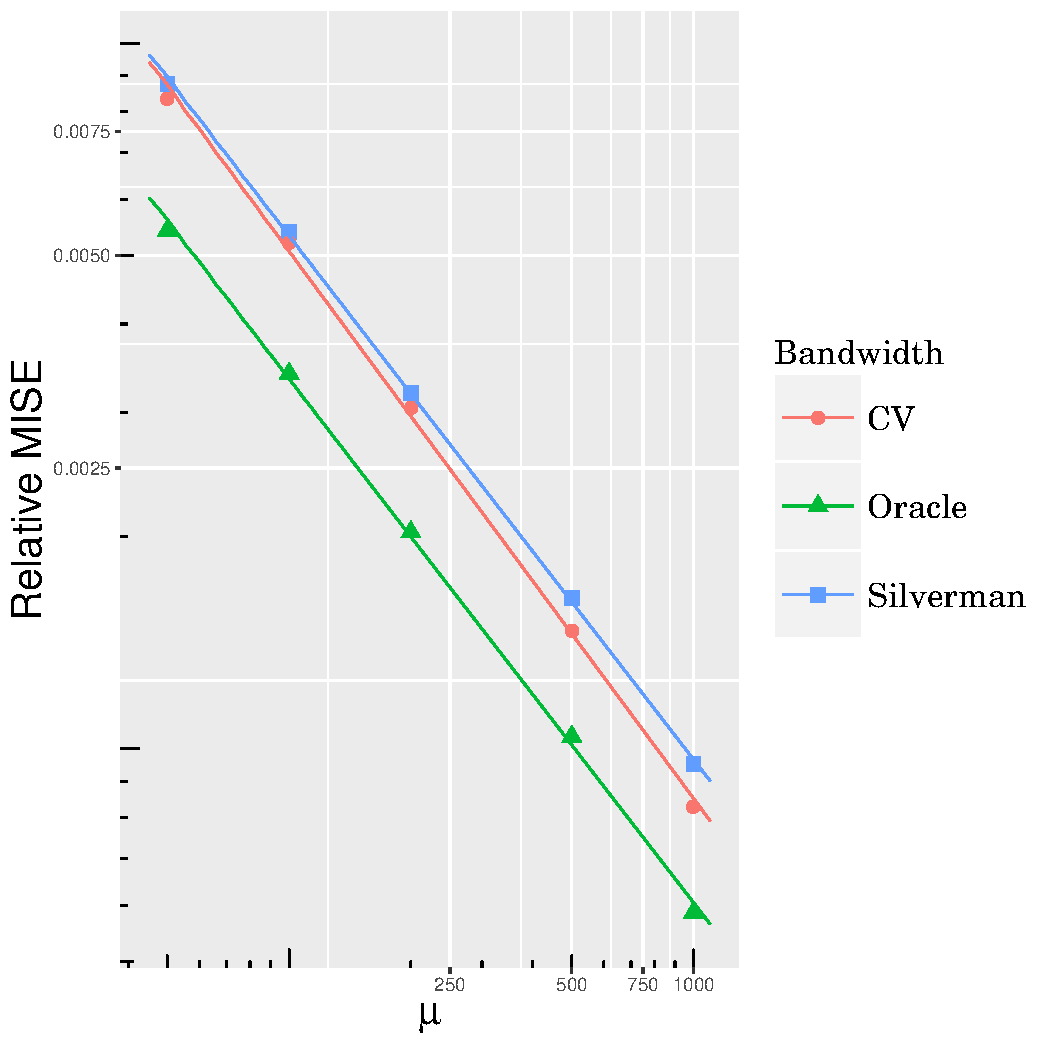
\includegraphics[width=\textwidth]{results/by_num_cases/RMISE-vs-cases-log-log}
    \caption{Relative MISE log-log}
    \label{fig:ise:unif_NCases_1h:c}
    \end{subfigure}
    \caption[MISE: by number of cases]{Mean Integrated Squared Error vs. number of cases}
    \label{fig:ise:unif_NCases_1h}
\end{figure}

\begin{figure}[htbp]
    \centering
    \begin{subfigure}[b]{0.3\textwidth}
    \includegraphics[width=\textwidth]{results/unif_100_1.0_1h/output/bandwidths-silverman}
    \caption{Silverman}
    \label{fig:bandwidths_x1:unif_100_1.0_1h:s}
    \end{subfigure}
    \begin{subfigure}[b]{0.3\textwidth}
    \includegraphics[width=\textwidth]{results/unif_100_1.0_1h/output/bandwidths-x1}
    \caption{Cross-validation, \(X_1\)}
    \label{fig:bandwidths_x1:unif_100_1.0_1h:x1}
    \end{subfigure}
    \begin{subfigure}[b]{0.3\textwidth}
    \includegraphics[width=\textwidth]{results/unif_100_1.0_1h/output/bandwidths-x2}
    \caption{Cross-validation, \(X_2\)}
    \label{fig:bandwidths_x1:unif_100_1.0_1h:x2}
    \end{subfigure}
    \caption{Bandwidth histograms for 100 incidents in a single peak from population of 10,000}
\end{figure}

\autoref{fig:one_sample:unif_NCases_1h} shows how one realization of incidents, distributed over the population, for sample sizes of 100 and 500.
This is done by multiplying the single-peak risk function by a constant in order to control the expected number of incidents per simulation.
\autoref{fig:ise:unif_NCases_1h} shows the effect on the MISE and RMISE:
\autoref{fig:ise:unif_NCases_1h:a} shows how MISE increases with expected incidents per patient.
One might expect the error to associated with estimating a function to \textit{decrease} as the number of incidents increases.
However, the expected number of incidents increases linearly with the intensity function value.
For example, double the number of incidents corresponds to an intensity of twice the value.
This makes comparing the MISE of estimates of intensity functions difficult, as the errors will also rise in the same direction.
In order to facilitate the comparison of intensity functions that have different expected number of incidents, we use the RMISE.
\autoref{fig:ise:unif_NCases_1h:b} shows how RMISE decreases with expected incidents per patient.
\autoref{fig:ise:unif_NCases_1h:c} is a log-log graph, showing a linear relationship between the logarithm of RMISE and the logarithm of the number of cases.
The values of the intercept and slope are -2.3525396 and -0.7316768 for the Oracle bandwidth; -1.8623772 and -0.7356884 for the Silverman bandwidth; and -1.5308541 and -0.8103349 for the cross-validation bandwidth.
The corresponding equations for RMISE are:

\begin{align}
    \mbox{RMISE}_{oracle} &= 0.09512727 N^{-0.7316768} \\
    \mbox{RMISE}_{silverman} &= 0.155303 N^{-0.7356884} \\
    \mbox{RMISE}_{cv} &= 0.2163508 N^{-0.8103349}
\end{align}

\textcolor{red}{TBD: chart of bandwidth vs. no. cases}

\begin{table}
\centering
\begin{tabular}{rrrr}
    \hline
    Decay Rate & Oracle & Silverman & CV \\ 
    \hline
    1.0 & -0.8180b & -0.7445 & 4.2668 \\
    1.4 & -0.7501 & -0.7224 & -0.5711 \\
    2.0 & -0.7548 & -0.7253 & -0.8425 \\
    \( \infty \) & -0.7317 & -0.7357 & -0.8103
\end{tabular}
\caption{Convergence power for different population decay rates}
\label{tab:convergence_vs_decay}
\end{table}

%%
%% Section
\section{Varying the sample size for fixed intensity}
\label{sec:results:unifNpop_1h}

%%%%%%%%%%%%%%%%%%%%%%%%%%%%%
% Parameter table
%%%%%%%%%%%%%%%%%%%%%%%%%%%%%
\begin{table}[htbp]
\centering
\begin{tabular}{ll}
\hline
Parameter & Value \\
\hline
Population size & 10,000, 20,000, 40,000, 60,000, 80,000, 100,000 \\
Population decay rate & uniform \\
Incident risk factor & 100, 200, 400, 600, 800, 1000 \\
Incident decay rate & 1.0 \\
Incident center & (0,0) \\
\hline
\end{tabular}
\caption{Parameters used for varying the sample size for fixed intensity}
\label{tab:params:unifNpop_1h}
\end{table}


We next examine the effect of increasing the sample size, while keeping the risk intensity function fixed.
In order to do this, we increase the population size and the expected number of incidents proportionately.
For this set of experiments, the population is uniformly distributed and the risk intensity has a single peak in the center with a fixed decay rate (standard deviation).

\begin{figure}[htbp]
    \centering
    \begin{subfigure}[b]{0.3\textwidth}
    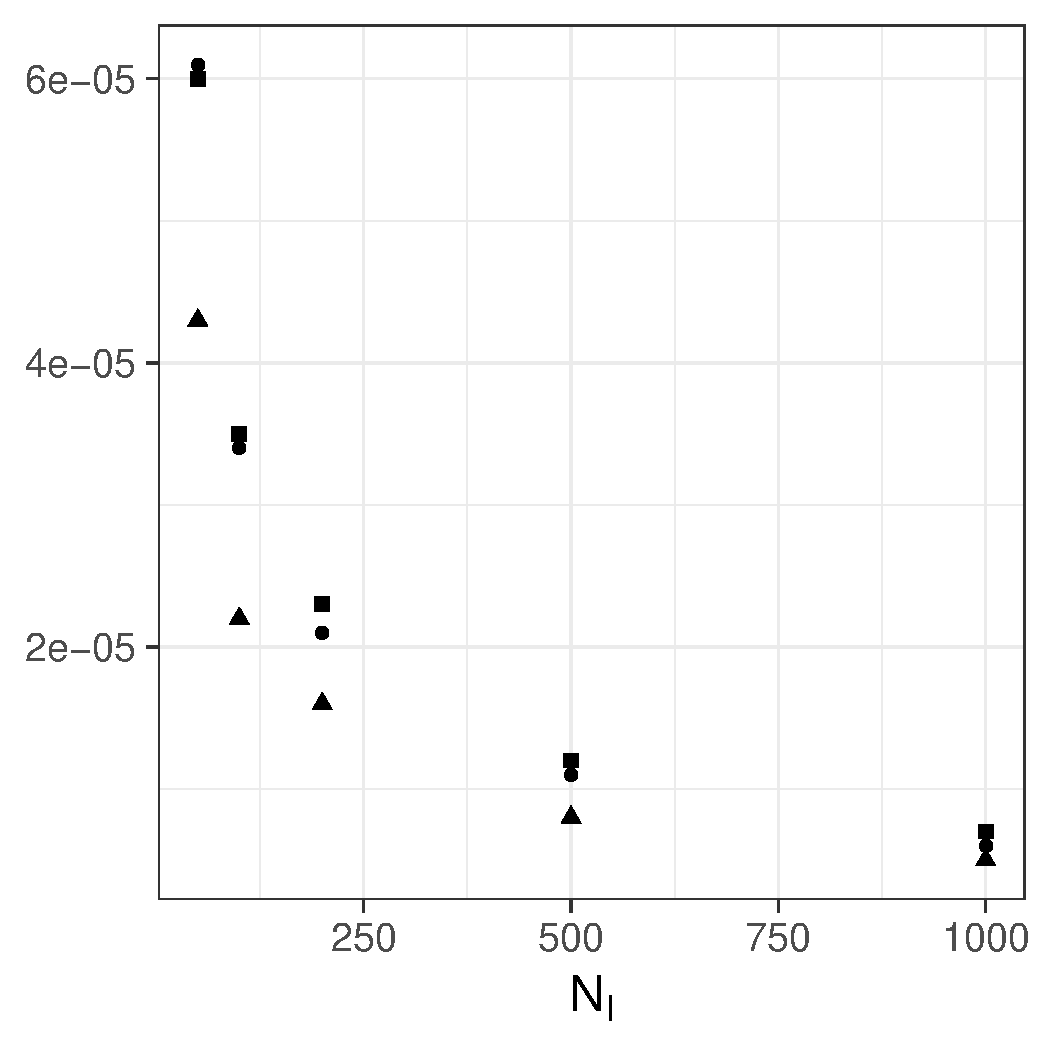
\includegraphics[width=\textwidth]{results/by_pop_size/MISE-vs-population}
    \caption{MISE}
    \end{subfigure}
    \begin{subfigure}[b]{0.3\textwidth}
    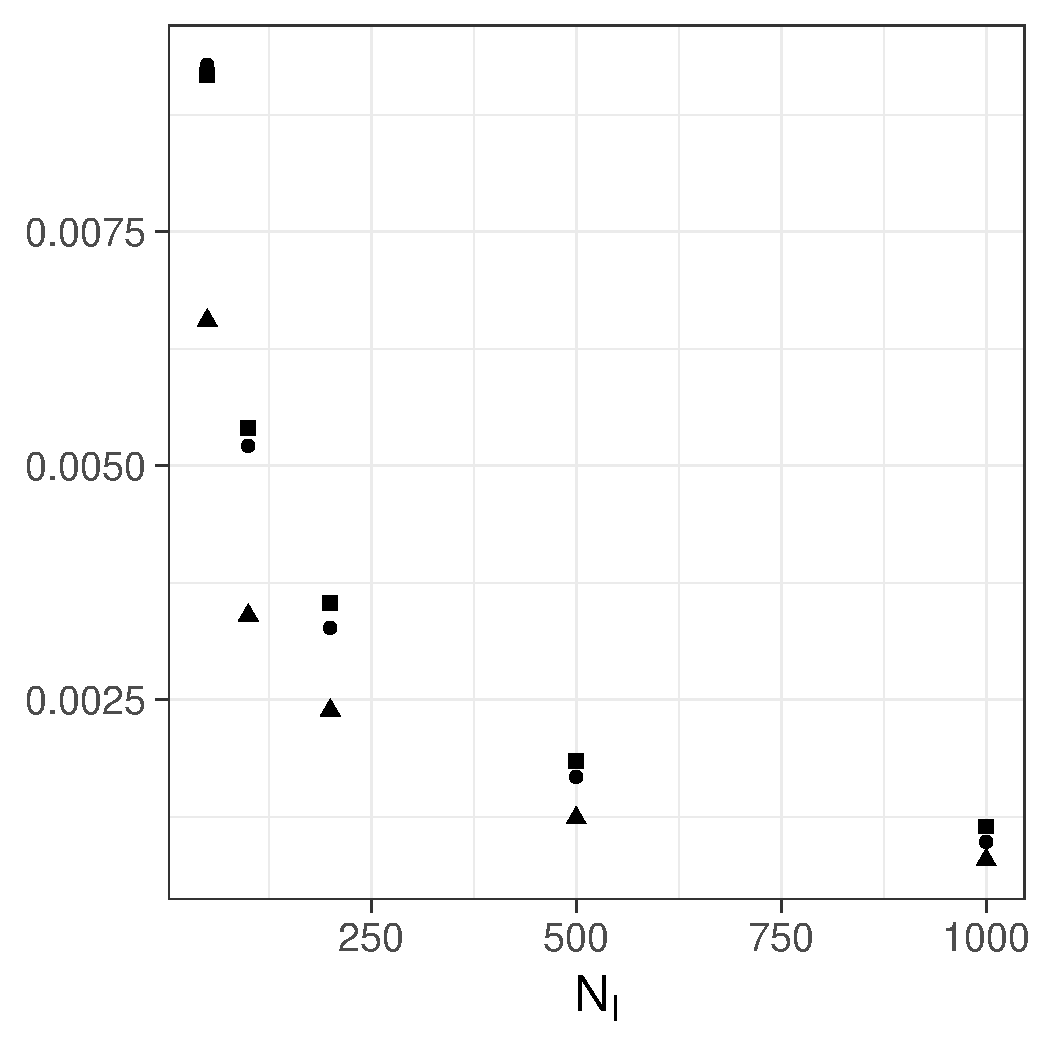
\includegraphics[width=\textwidth]{results/by_pop_size/RMISE-vs-population}
    \caption{Relative MISE}
    \end{subfigure}
    \begin{subfigure}[b]{0.3\textwidth}
    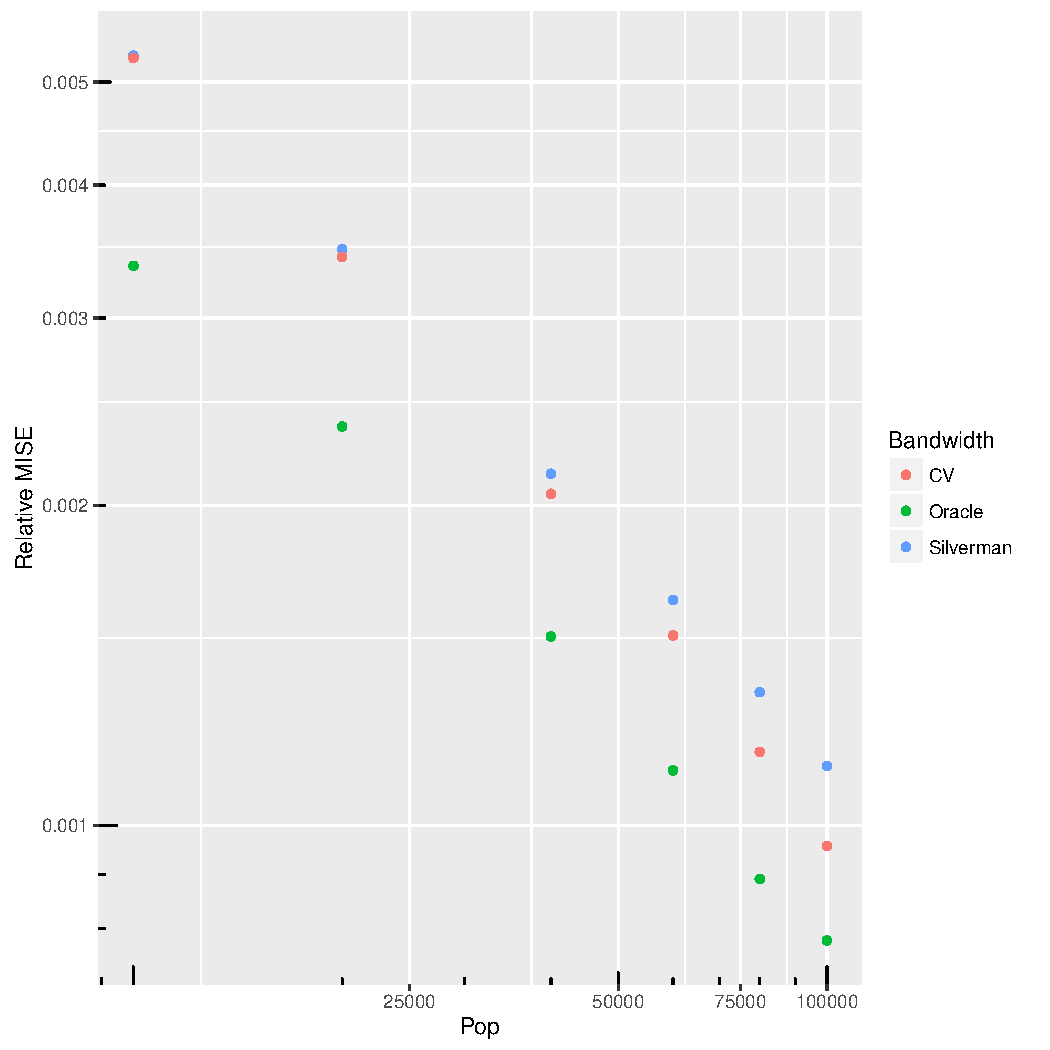
\includegraphics[width=\textwidth]{results/by_pop_size/RMISE-vs-population-log-log}
    \caption{Relative MISE log-log}
    \end{subfigure}
    \caption[MISE: by population size]{Mean Integrated Squared Error vs. population size}
    \label{fig:ise:unifNpop_1h}
\end{figure}


%%
%% Section
\section{Varying the decay of the risk function}
\label{sec:results:unif_100_SD}

%%%%%%%%%%%%%%%%%%%%%%%%%%%%%
% Parameter table
%%%%%%%%%%%%%%%%%%%%%%%%%%%%%
\begin{table}[htbp]
\centering
\begin{tabular}{ll}
\hline
Parameter & Value \\
\hline
Population size & 10,000 \\
Population decay rate & uniform \\
Incident risk factor & 100 \\
Incident decay rate & 0.7, 1.0, 1.4, 2.0 \\
Incident center & (0,0) \\
\hline
\end{tabular}
\caption{Parameters used for varying the decay rate of the risk function}
\label{tab:params:unif_100_SD}
\end{table}

In this section, we compare the effect of the decay rate of the risk function on the estimate.
The population distribution is uniform, and the expansion factor remains constant at 100, but
the standard deviation of the Gaussian risk function is varied.

\begin{figure}[htbp]
    \centering
    \begin{subfigure}[b]{0.3\textwidth}
    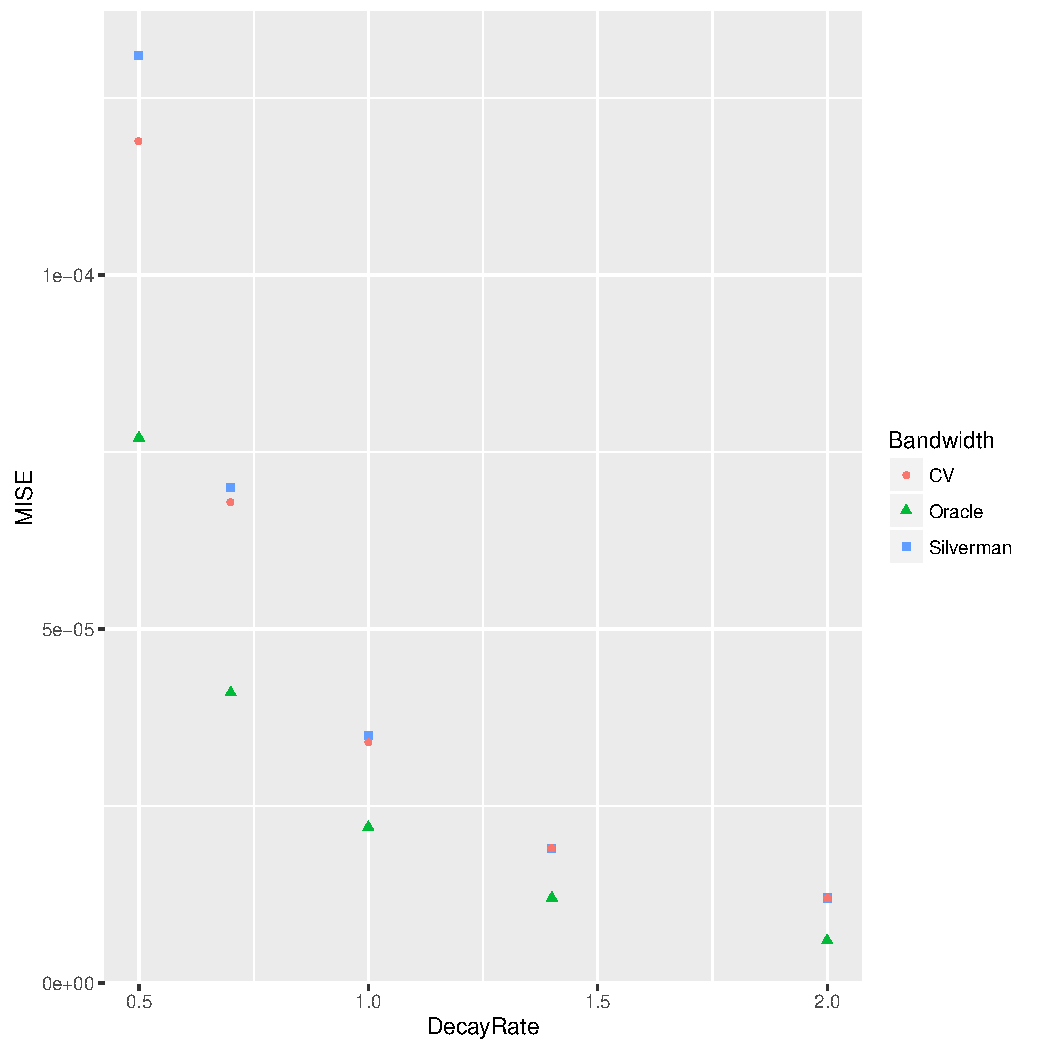
\includegraphics[width=\textwidth]{results/by_cases_decay/MISE-vs-risk-decay}
    \caption{MISE}
    \end{subfigure}
    \begin{subfigure}[b]{0.3\textwidth}
    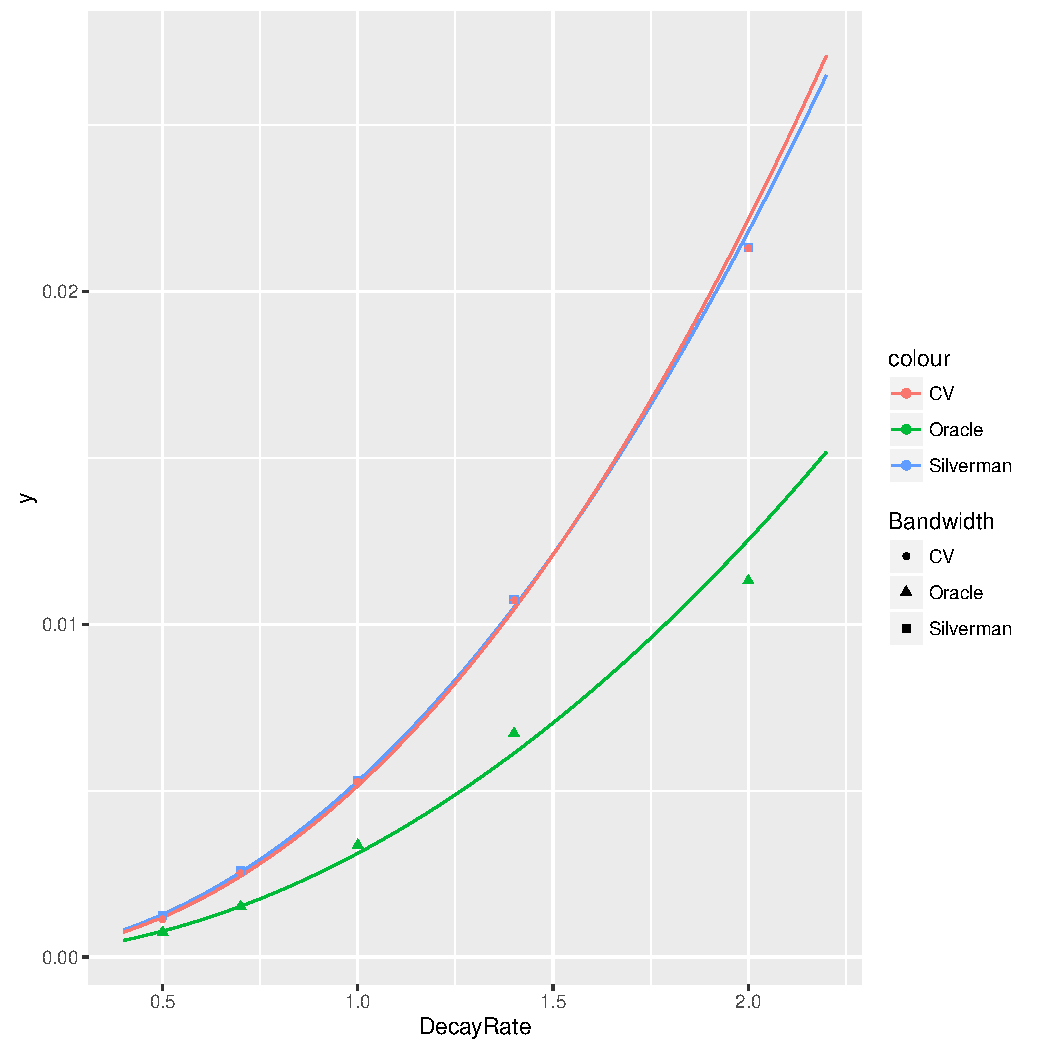
\includegraphics[width=\textwidth]{results/by_cases_decay/RMISE-vs-risk-decay}
    \caption{Relative MISE}
    \end{subfigure}
    \begin{subfigure}[b]{0.3\textwidth}
    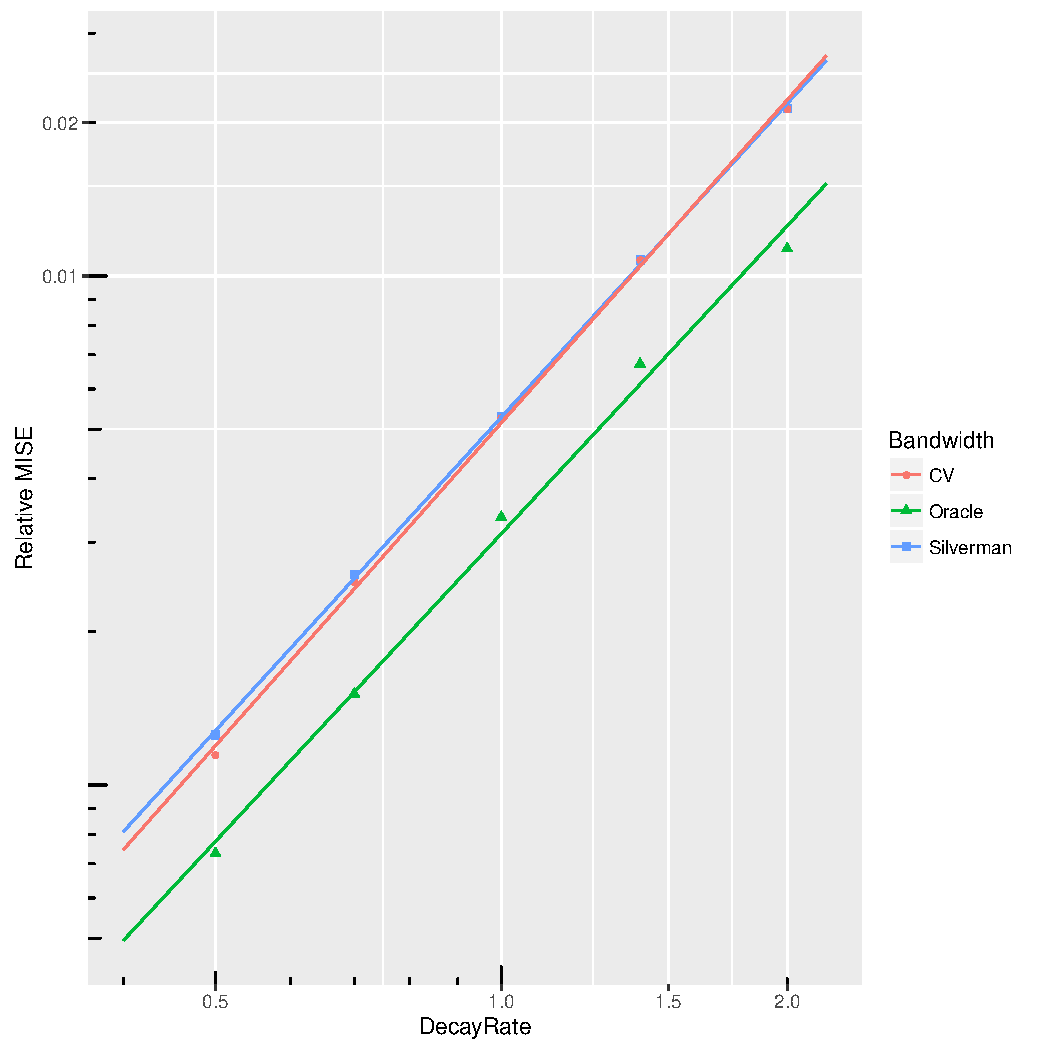
\includegraphics[width=\textwidth]{results/by_cases_decay/RMISE-vs-risk-decay-log-log}
    \caption{Relative MISE log-log}
    \end{subfigure}
    \caption[MISE: by risk decay]{Mean Integrated Squared Error vs. risk decay rate}
    \label{fig:ise:unif_100_SD}
\end{figure}

%%
%% Section
\section{Varying the decay of the population density}
\label{sec:results:pSD_100_1h}

In this section, we compare the effect of different population distributions on the estimation of a single, fixed risk function.
The population s
The risk function has an expansion factor of 100.

\begin{table}[htbp]
\centering
% latex table generated in R 3.3.3 by xtable 1.8-2 package
% Sun Apr  8 13:54:46 2018
\begin{tabular}{lrrr}
  \toprule
 & Oracle & Silverman & CV \\ 
  \midrule
MISE & 0.001480 & 0.001468 & 0.001755 \\ 
  Relative MISE & 0.226751 & 0.224963 & 0.268930 \\ 
  Normalized MISE & 147.969414 & 146.802375 & 175.493859 \\ 
  MIAE & 0.006271 & 0.006336 & 0.006678 \\ 
  Relative MIAE & 0.077623 & 0.078435 & 0.082665 \\ 
  Normalized MIAE & 0.000063 & 0.000063 & 0.000067 \\ 
  Supremum error & 0.405078 & 0.434458 & 0.405401 \\ 
  Normalized Sup error & 0.004051 & 0.004345 & 0.004054 \\ 
  Peak bias & 0.331304 & 0.360895 & 0.330921 \\ 
  Relative Peak bias & 4.101243 & 4.467549 & 4.096503 \\ 
  Peak drift & 2.223677 & 2.215194 & 2.274708 \\ 
  Relative Peak drift & 0.317668 & 0.316456 & 0.324958 \\ 
  Centroid bias & -0.008225 & -0.006728 & -0.011830 \\ 
  Relative Centroid bias & -0.101821 & -0.083283 & -0.146446 \\ 
  Centroid drift & 0.325701 & 0.299465 & 0.400859 \\ 
  Relative Centroid drift & 0.046529 & 0.042781 & 0.057266 \\ 
   \bottomrule
\end{tabular}

\caption{Error rates for uniform population of 10,000, single peak intensity of factor 100 and decay rate 0.7}
\label{tab:results:p0.7_100_1.0_1h}
\end{table}


\begin{figure}[htbp]
    \centering
    \begin{subfigure}[b]{0.3\textwidth}
    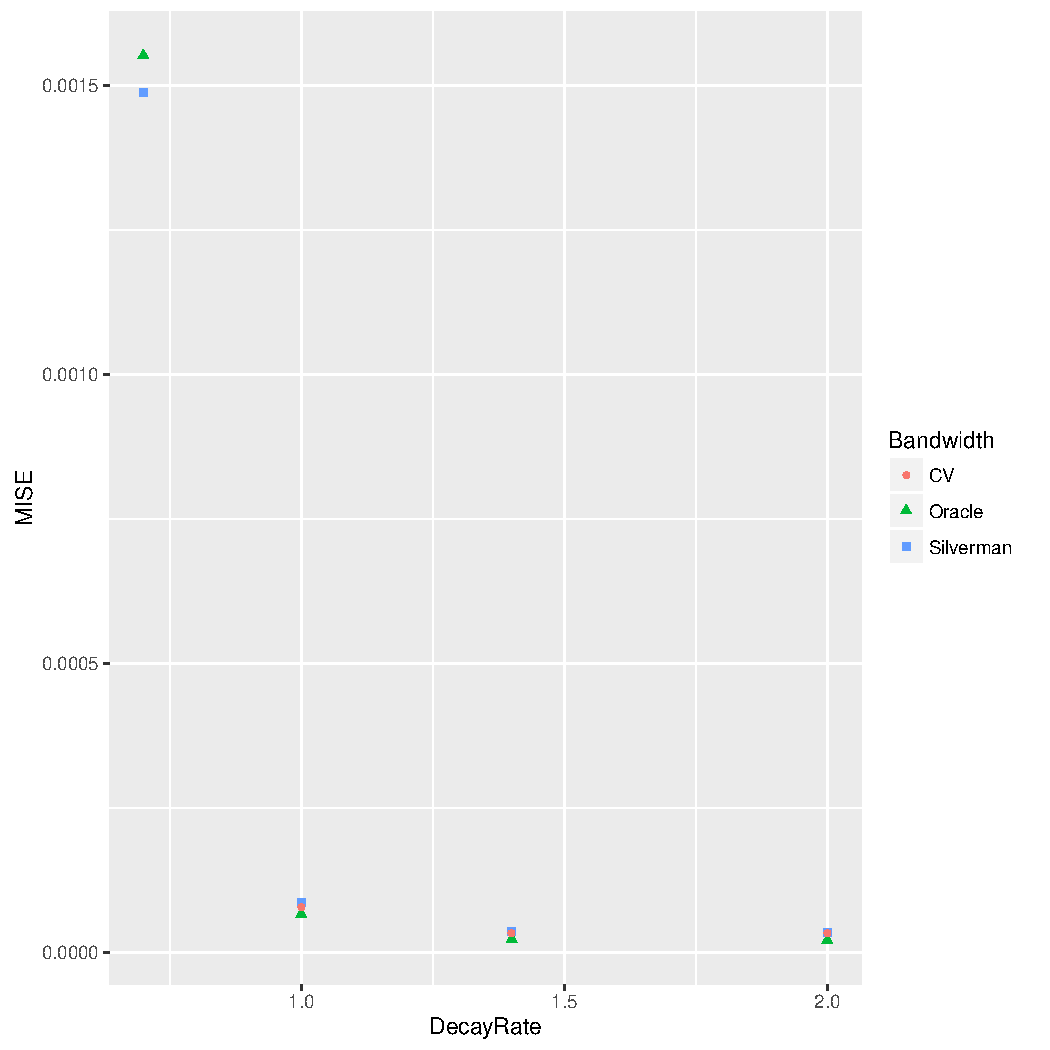
\includegraphics[width=\textwidth]{results/by_population_decay/MISE-vs-population-decay}
    \caption{MISE}
    \end{subfigure}
    \begin{subfigure}[b]{0.3\textwidth}
    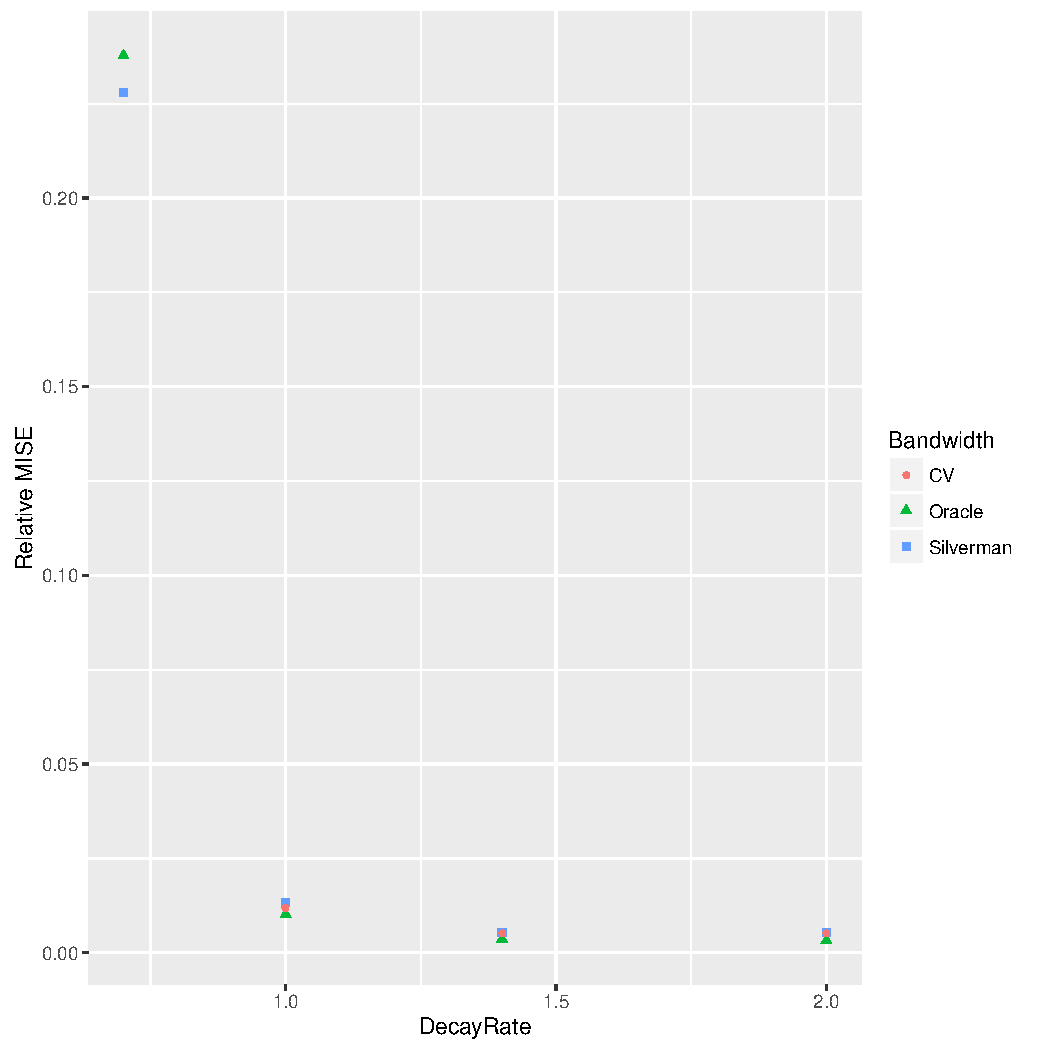
\includegraphics[width=\textwidth]{results/by_population_decay/RMISE-vs-population-decay}
    \caption{Relative MISE}
    \end{subfigure}
    \begin{subfigure}[b]{0.3\textwidth}
    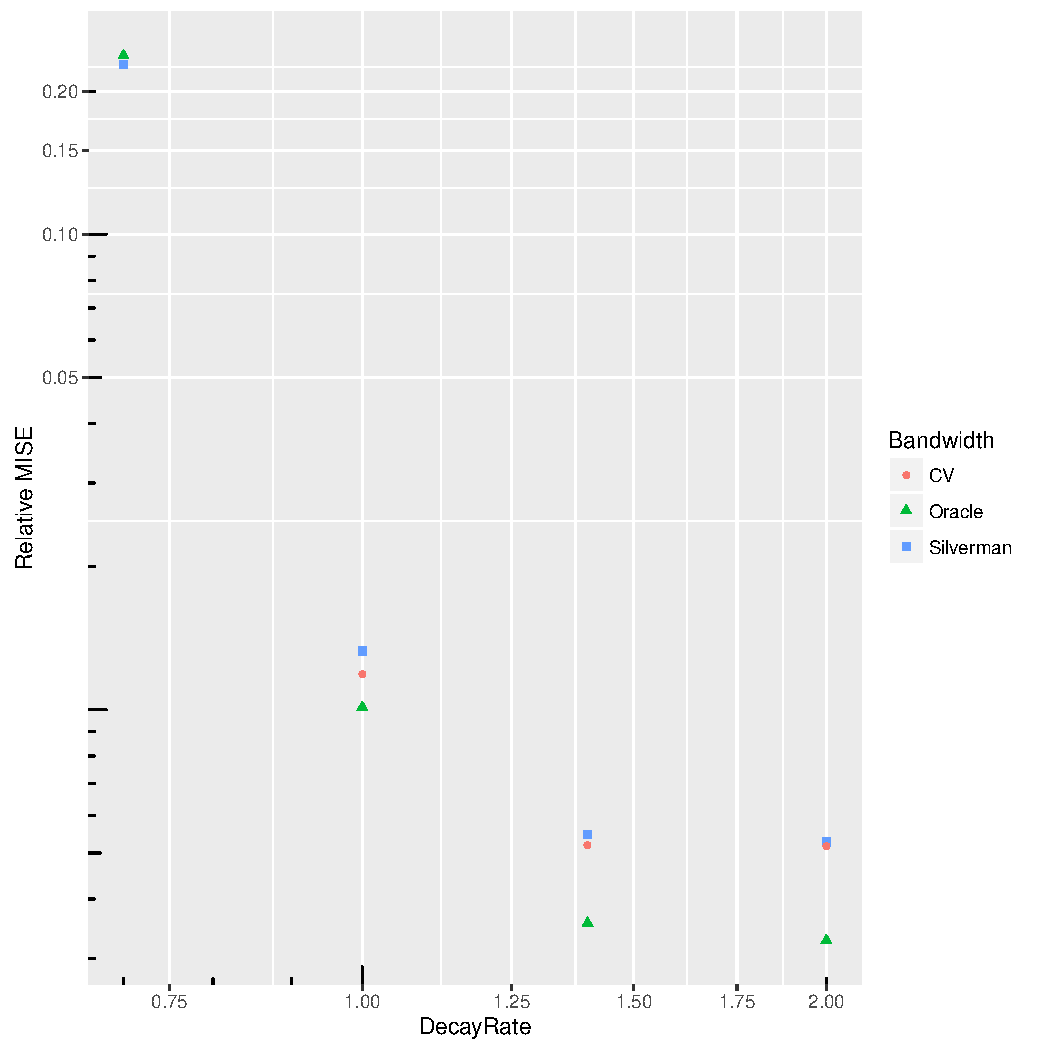
\includegraphics[width=\textwidth]{results/by_population_decay/RMISE-vs-population-decay-log-log}
    \caption{Relative MISE log-log}
    \end{subfigure}
    \caption[MISE: by risk decay]{Mean Integrated Squared Error vs. population decay rate}
    \label{fig:ise:pSD_100_1h}
\end{figure}


%%
%% Section
\section{Varying the distance between two peaks}
\label{sec:results:p1.4_100_G}

\begin{figure}[htbp]
    \centering
    \begin{subfigure}[b]{0.3\textwidth}
    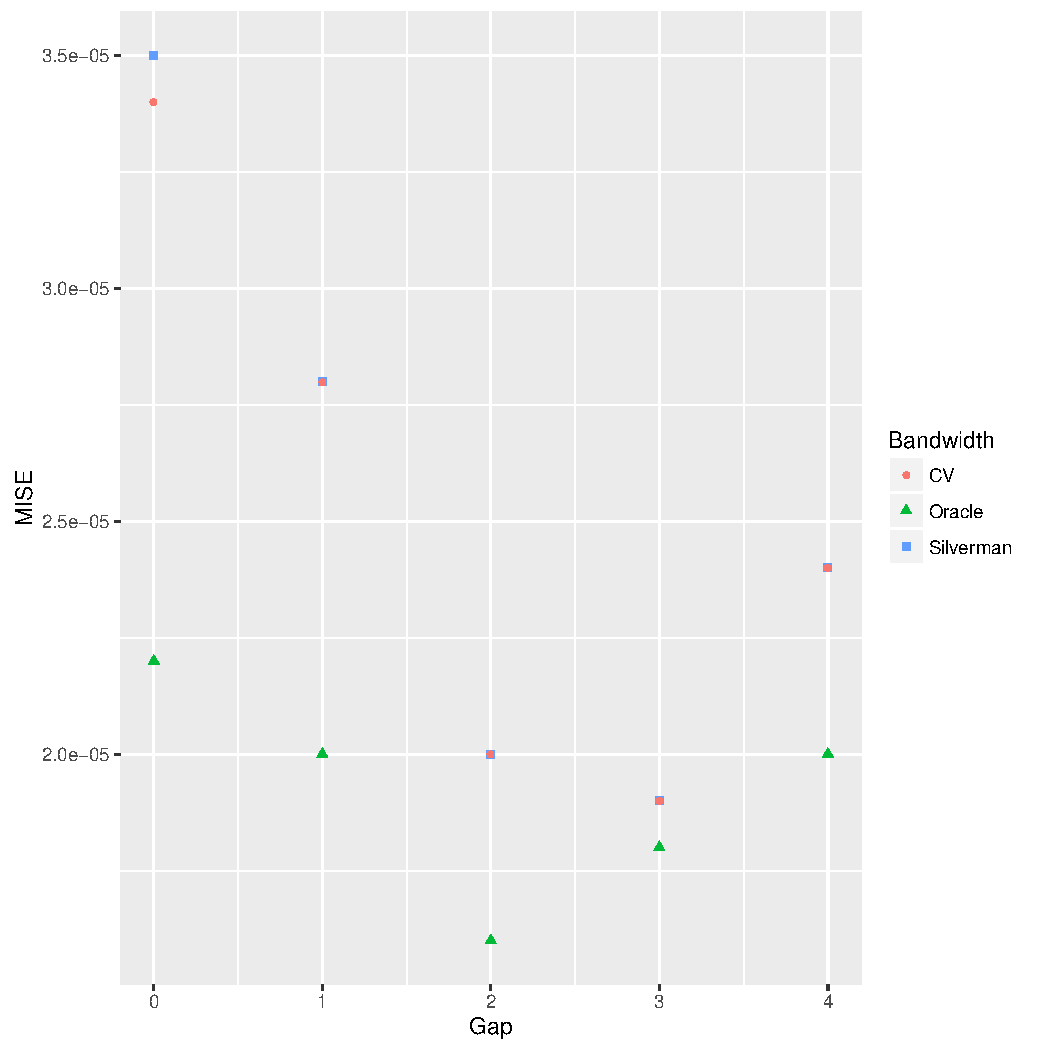
\includegraphics[width=\textwidth]{results/by_two_peaks/MISE-vs-risk-peak-gap}
    \caption{MISE}
    \end{subfigure}
    \begin{subfigure}[b]{0.3\textwidth}
    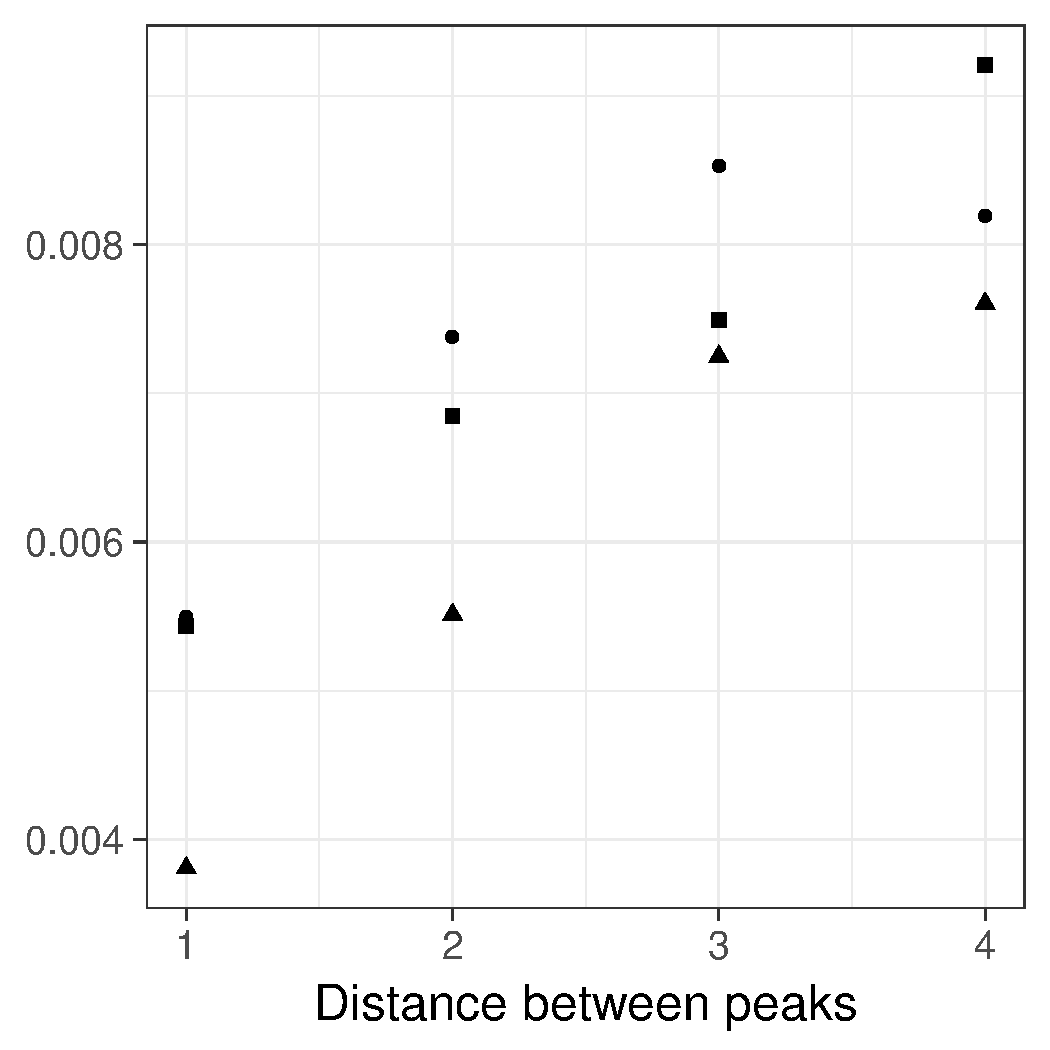
\includegraphics[width=\textwidth]{results/by_two_peaks/RMISE-vs-risk-peak-gap}
    \caption{Relative MISE}
    \end{subfigure}
    \begin{subfigure}[b]{0.3\textwidth}
    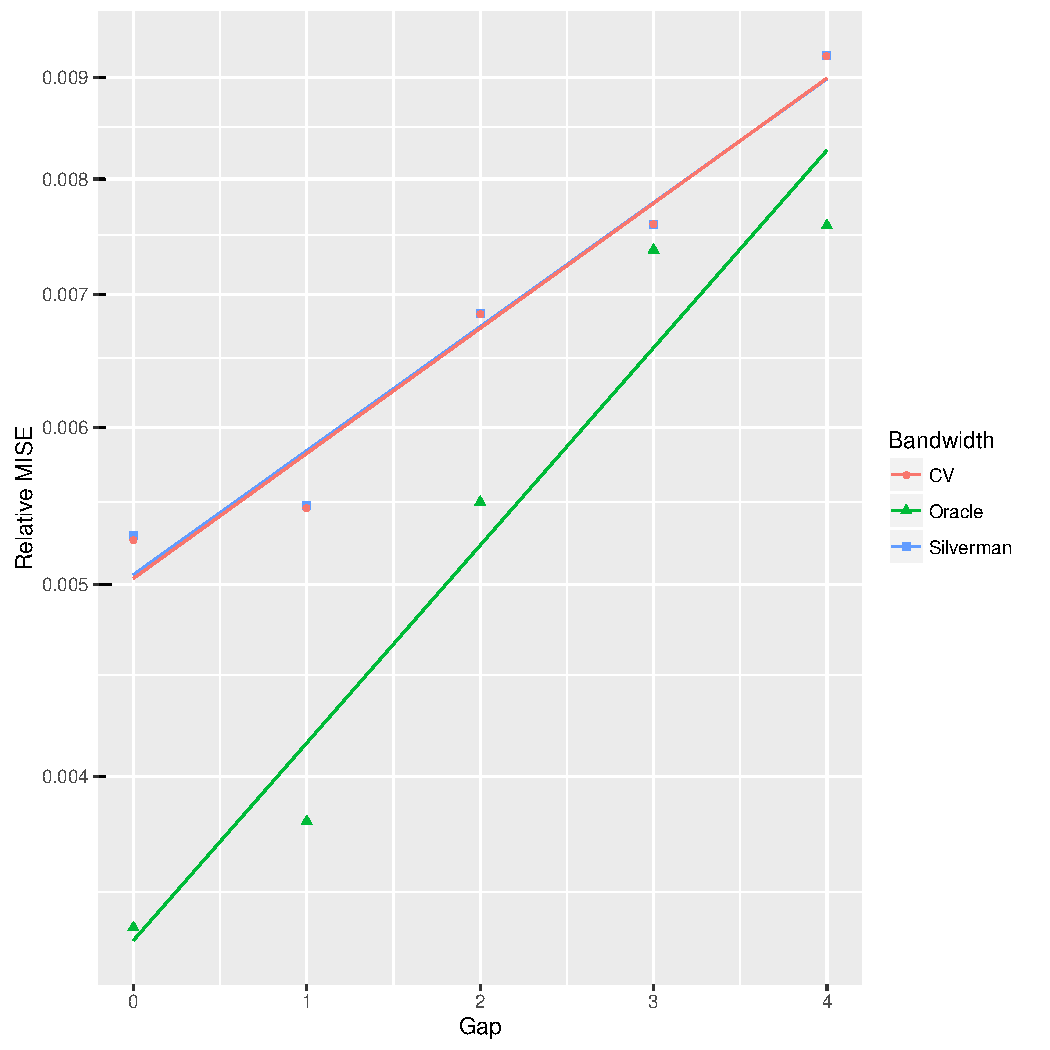
\includegraphics[width=\textwidth]{results/by_two_peaks/RMISE-vs-risk-peak-gap-log-log}
    \caption{Relative MISE log-log}
    \end{subfigure}
    \caption[MISE: by risk decay]{Mean Integrated Squared Error vs. distance between two risk peaks}
    \label{fig:ise:p1.4_100_G}
\end{figure}

%%
%% Section
\section{Varying the distance between the population and risk function peaks}
\label{sec:ise:p1.4_Gap_risk}

\begin{figure}[htbp]
    \centering
    \begin{subfigure}[b]{0.3\textwidth}
    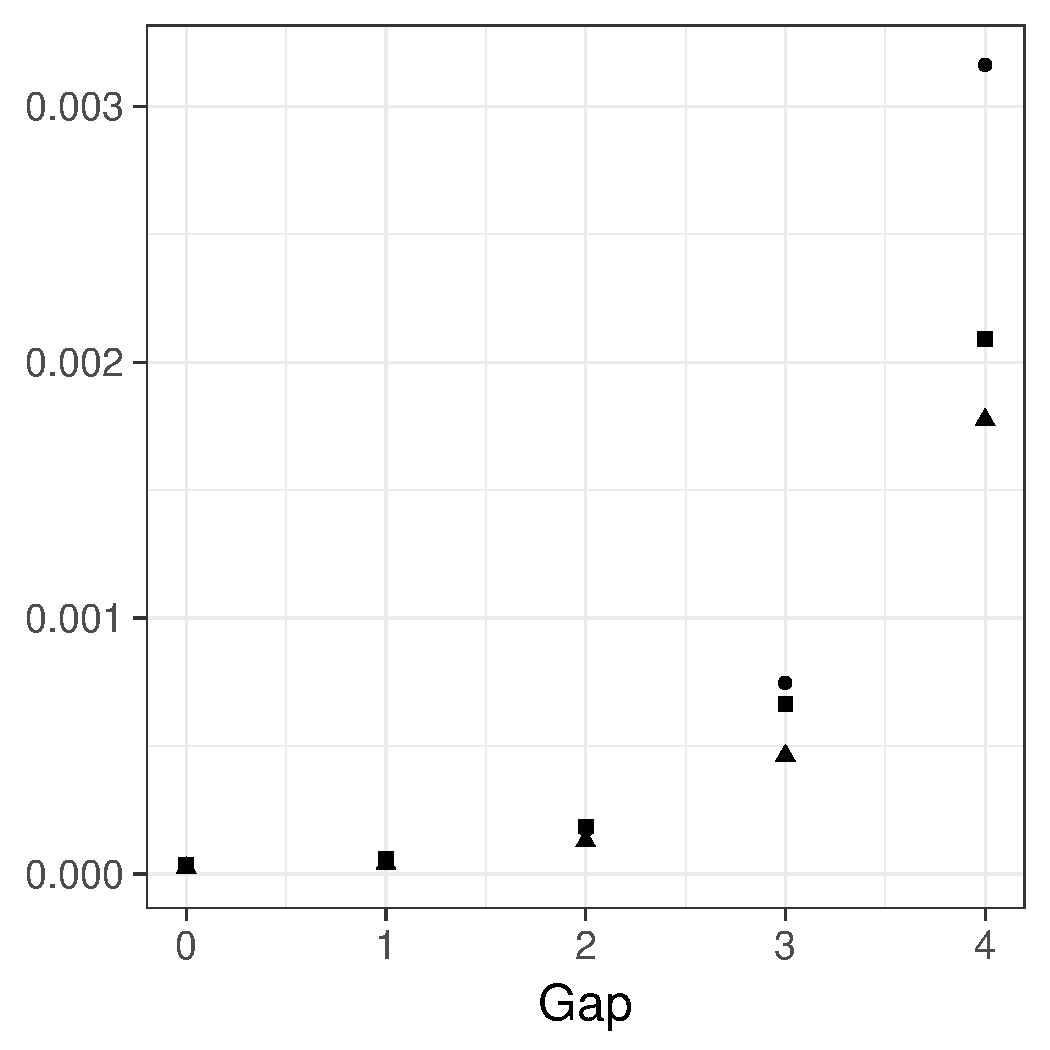
\includegraphics[width=\textwidth]{results/by_pop_risk_distance/MISE-vs-population-risk-gap}
    \caption{MISE}
    \end{subfigure}
    \begin{subfigure}[b]{0.3\textwidth}
    \includegraphics[width=\textwidth]{results/by_pop_risk_distance/RMISE-vs-population-risk-gap}
    \caption{Relative MISE}
    \end{subfigure}
    \begin{subfigure}[b]{0.3\textwidth}
    \includegraphics[width=\textwidth]{results/by_pop_risk_distance/RMISE-vs-population-risk-gap-log-log}
    \caption{Relative MISE log-log}
    \end{subfigure}
    \caption[MISE: by risk decay]{Mean Integrated Squared Error vs. distance between population and risk peaks}
    \label{fig:ise:p1.4_Gap_risk}
\end{figure}

%%
%% Discussion
%%

\section{Discussion}
\label{sec:discussion}

We are investigating the effectiveness of the DKD in estimating functions that return the incidence risk of chronic diseases. 
The DKD is computed by taking a kernel estimate of the disease incidence intensity and dividing by a kernel estimate of the population density at any given point.
We used several methods to estimate the error of the DKD estimate.
We ran several scenarios to examine how variations in the incidence risk function, the population, and the sample size affect the accuracy of the estimation. 

First, we varied the multiplication factor of the risk function.
Effectively, this resulted in increasing the number of incidents, while keeping the population constant.
This is analogous to having a greater risk of getting a disease.
We observed that the absolute mean integrated squared error rose as the number of incidents increased.
However, the relative mean integrated squared error fell with increasing the multiplication factor, in a negative polynomial order.

Second, we varied the number of incidents and the population by the same proportion.
The risk function was kept the same.
This is analogous to extending the time frame of the study.
We observed that both the absolute and relative mean integrated squared error fell with increasing the number of incidents, in a negative polynomial order.

\[
    \mbox{RMISE} = K n^{\alpha}
\]


\begin{table}[htbp]
\begin{tabular}{l*6c}
  \hline
  & \multicolumn{2}{c}{Oracle} & \multicolumn{2}{c}{Silverman} & \multicolumn{2}{c}{CV} \\ 
  decay & K & \( \alpha \) & K & \( \alpha \) & K & \( \alpha \) \\ 
  \hline
  0.7000 & -5.1305 & -0.3011 & -3.9831 & -0.4310 & -3.9296 & -0.4545 \\ 
  1.0000 & -2.3525 & -0.7317 & -1.8624 & -0.7357 & -1.5309 & -0.8103 \\ 
  1.4000 & -1.9569 & -0.6657 & -1.3159 & -0.7012 & -1.2255 & -0.7216 \\ 
  2.0000 & -1.6753 & -0.6036 & -0.8370 & -0.6518 & -0.7970 & -0.6609 \\ 
  \( \infty \) & -0.6438 & -0.3273 & -0.3175 & -0.3774 & -0.3170 & -0.3775 \\ 
  \hline
\end{tabular}
\end{table}

\graphicspath{{./}}
